\documentclass{article}
\usepackage[utf8]{inputenc}
\usepackage[margin=2cm]{geometry}
\usepackage{fullpage,enumitem,amssymb,amsmath,xcolor,cancel,gensymb}
\usepackage{graphicx}
\usepackage{caption}
\usepackage{subcaption}
\usepackage{indentfirst}
\usepackage{fixltx2e}
\usepackage{hyperref}
\usepackage{listings}
\usepackage{tabularx}
\usepackage{booktabs}
\usepackage{wrapfig}
\setlength{\parskip}{1em}
\usepackage[T1]{fontenc}
\usepackage{imakeidx}
\makeindex[columns=3, title=Alphabetical Index, intoc]
\usepackage{float}
\usepackage{comment}

\usepackage{listings}
\usepackage{xcolor}

\definecolor{codegreen}{rgb}{0,0.6,0}
\definecolor{codegray}{rgb}{0.5,0.5,0.5}
\definecolor{codepurple}{rgb}{0.58,0,0.82}
\definecolor{backcolour}{rgb}{0.95,0.95,0.92}

\lstdefinestyle{mystyle}{
    backgroundcolor=\color{backcolour},   
    commentstyle=\color{codegreen},
    keywordstyle=\color{magenta},
    numberstyle=\tiny\color{codegray},
    stringstyle=\color{codepurple},
    basicstyle=\ttfamily\footnotesize,
    breakatwhitespace=false,         
    breaklines=true,                 
    captionpos=b,                    
    keepspaces=true,                 
    numbers=left,                    
    numbersep=5pt,                  
    showspaces=false,                
    showstringspaces=false,
    showtabs=false,                  
    tabsize=2
}

\lstset{style=mystyle}

%%
%% Minted listings support 
%% Need pygment <http://pygments.org/> <http://pypi.python.org/pypi/Pygments>
\usepackage{minted}
%% auto break lines
\setminted{breaklines=true}
\usepackage{natbib}
\usepackage{xurl}

%\begin{align*}…\end{align*} if you want to fit an equation. 
%FOR PICTURES: include graphicsx 
%\includegraphics[scale=x]{name}
%double space and write caption in the center classshe 

\title{\textbf{Elective In Artificial Intelligence - HRI and RA}\\\textbf{RushHour: A Collaborative Social Robot}}
\author{Alessio Sfregola 1798423 \\ Caterina Borzillo 1808187 \\ Federica Cocci 1802435}
\date{March 15th, 2023}


\begin{document}

\maketitle

\begin{figure}[!htbp]
\centering

\includegraphics[width=0.4\textwidth]{images/logo-sapienza.png}
\\

\includegraphics[width=0.4\textwidth]{images/scritta-sapienza.png}
\label{fig:largenenough}
\end{figure}

\\
\begin{center}
All authors have contributed to the project in an equal way.
\end{center}

\newpage

\tableofcontents

\newpage

\section{Abstract}
RushHour is a social and interactive robot for people's entertainment. He plays with the human the Rush Hour game in a collaborative way: human and robot work together to reach the goal making one move alternately. The social interaction consists in an introductory presentation, in an initial and final surveys and in different robot animations also during the game. The robot reasoning aspect is developed through AIPlan4EU framework. The physical communication between the several components of the project has been developed using a system of clients and servers.

%* introduction: your idea about the project, purpose of the project, a brief summary of what you have actually developed, why you think the problem you faced in your project is important, motivation for using both HRI and RA techniques.
\section{Introduction}
Artificial Intelligence (AI) and social robots are rapidly transforming the way we interact with technology and with each other. Social robots are machines designed to simulate human behavior and communication, often through the use of AI. These robots can take many forms, such as humanoid robots, pet robots, or virtual assistants, and they are increasingly being used in a variety of settings, including homes, schools, hospitals, and public spaces.
\noindent The potential benefits of social robots are numerous. They can provide companionship for the elderly, assist individuals with disabilities, and support children's education and development. They can also perform tasks that are dangerous or repetitive for humans, such as cleaning or manufacturing. Furthermore, they can be used to collect data and perform analysis in areas such as healthcare and transportation, leading to better decision-making and outcomes. In our case, we want that our social robot, in addition to experiencing the social field with the human, is also equipped with intellectual abilities that enable it to reason and solve the game along with the human.
\noindent The way the overall interaction is established is very important regarding the acceptability aspect of the human towards the robot. The rise of social robots has to deal, in fact, also with this aspect: how to make the robot behave toward the human so that the human has the best possible experience. 
\noindent Overall, the integration of AI and social robots in society has the potential to revolutionize our lives in positive ways, but it is important to carefully consider the implications and ensure that these technologies are developed and used responsibly.

\indent The basis idea of our project is to develop a robot, called RushHour, that solve the Rush Hour game cooperating with the human. Rush Hour \ref{fig:rush_hour} is a sliding puzzle game whose objective is to move a red car through a grid of other cars and trucks to the exit of the game board. Here are the basic rules of the game: the game board consists of a 6x6 grid of squares where cars (length 2) and trucks (length 3) are placed vertically or horizontally; the player moves the cars and trucks by sliding them along the grid horizontally or vertically, but not diagonally in order to clear a path for the red car to reach the exit, which is located on the edge of the grid opposite the starting position. In our version of Rush Hour, a move corresponds to a sequence of movements all in the same direction relative to the same vehicle: man and robot take turns at the board each time a different vehicle moves or the direction of the movement of the same vehicle changes.
\noindent These rules brought us to develop the reasoning ability of the robot in order to let him calculate the best next move allowing it to win the match in the fastest way possible, taking into account the configuration of the board and its changes once the human makes a move. \\
\indent The reasoning aspect of our project has been implemented using a Python framework called AIPlan4EU \cite{aiplan4eu} where, in order to define a planning problem, we have to declare different types of objects, fluents, actions with their preconditions and effects, initial state and goal.\\
\indent Concerning human-robot interaction (HRI), we want to get the interaction between human and robot as natural as possible. The idea is to use our software on a physical robot called Pepper \cite{pepper} which is from the NAOqi robots family \cite{naoqi} \ref{fig:naoqi_family}.
For this purpose, NAOqi has been used as it provides APIs, for example for speech recognition and synthesis capabilities, that allows the robot to understand and respond to spoken commands and to communicate with users through speech. It also includes a range of sensors, such as cameras and microphones, that enable Pepper to perceive and interact with its environment. One key aspect of NAOqi that makes it well-suited for human-robot interaction is its modular architecture. The platform is designed to be easily extensible, allowing developers to add new behaviors and capabilities to the robot as needed.
\noindent Actually we have tested our software only on a simulated Pepper \ref{fig:choregraphe}. In the simulated environment the robot can act as if he was physical. We use Choregraphe Suite \cite{choregraphe} as platform for the simulation. In Choregraphe some of the tools of the physical NAOqi are not enable such as sonars or verbal speaking but we have find some expediences to test however our code for the sensing part.
\noindent The way the robot is represented in its naturalness is crucial for the success of the human's experience with the robot. The fact that the robot, after having introduced itself with the human, learns his name and continues to interact with him using the user's name, gives a sense of familiarity and welcome in the human's mind and this is fundamental in those situations in which, for example, there is a robot that has to deal with children (educational field) or elderly people that have in some way start a process of "acceptability" of the robot in order to interact with him in the correct way.\\ 
\indent Thanks to JavaScript (JS) and CSS and HTML, we created a web application to reproduce the Pepper tablet. This web application allows the user and the robot play together since the human can visualize the progress of the game and play the next move for solving the problem. Finally, in order to make all these components communicate with each other, we have exploited websockets and in order to implement them in Python we have used Tornado \cite{tornado}. 

\begin{figure}[H]
    \centering
    \begin{subfigure}{.33\textwidth}
      \centering
      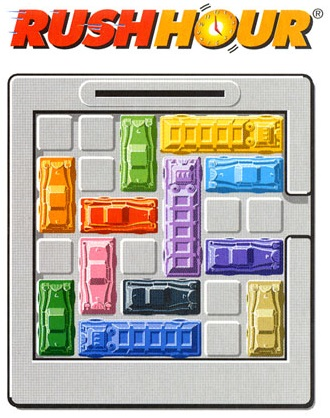
\includegraphics[width=0.5\linewidth]{images/rushhour.jpg}
      \caption{Rush Hour}
      \label{fig:rush_hour}
    \end{subfigure}%
    \begin{subfigure}{.33\textwidth}
      \centering
      
\includegraphics[width=0.6\linewidth]{images/naoqi_fam1.png}
      \caption{NAOqi family}
      \label{fig:naoqi_family}
    \end{subfigure}
    \begin{subfigure}{.33\textwidth}
      \centering
      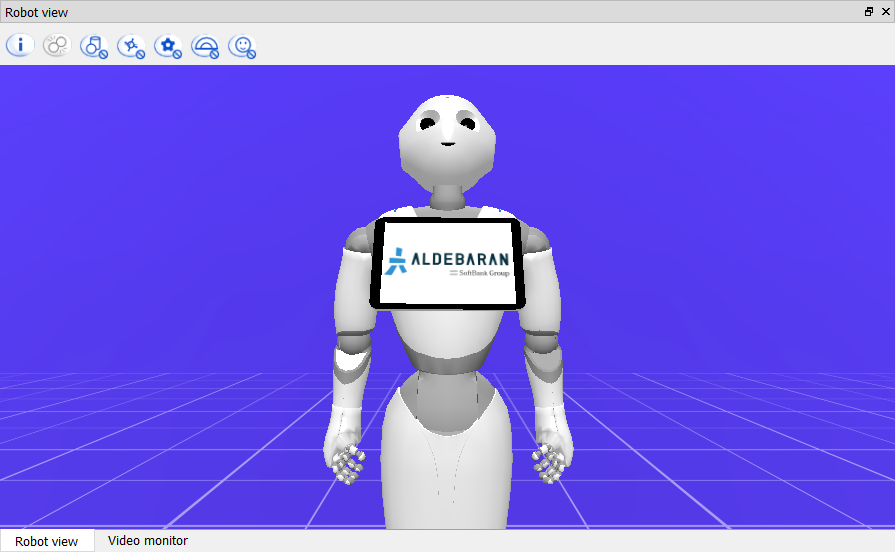
\includegraphics[width=0.85\linewidth]{images/pepper_choregraphe.png}
      \caption{Virtual Pepper in Choregraphe}
      \label{fig:choregraphe}
    \end{subfigure}
    \caption{Rush Hour and Robots}
\end{figure}

%* related work: papers you have read that are related to your project (including the ones you presented, the ones mentioned during the lectures, etc.) and the relation between these papers and your project. Include one section about HRI and one section about RA.
\section{Related Works}
\indent Social robots that play games are an emerging field of robotics that is rapidly gaining popularity. These robots are designed to interact with humans in a social setting and engage in various games with them, such as board games, card games, and video games \ref{fig:interactions}. The primary goal of these robots is to provide entertainment and companionship to humans, while also promoting social interaction and cognitive development. With advances in artificial intelligence and robotics, social robots are becoming more sophisticated and capable of adapting to individual human behavior. This has led to an increasing interest in the potential applications of social robots in areas such as education, therapy, and elderly care. Overall, social robots that play games are a fascinating and exciting development in the field of robotics, with the potential to transform the way we interact with technology and each other.
\subsection{Human-Robot Interaction}
\indent Among the researchers that for decades are making great contributions to HRI field there is certainly the prominent researcher Rachid Alami, head of the Robotics and Artificial Intelligence group at LAAS-CNRS in Toulouse, France. Alami research field concerns the way robots can work and interact together with humans in real-world environments. His studies focus on one side on the development of intelligent robots that are capable of performing complex tasks in unstructured environments, such as homes, hospitals, and factories and on the other side on the development of robots that can understand and respond to human gestures and speech, making them more natural and intuitive and that for example can be used in fields such as human-robot collaboration, assistive robotics, and social robotics. For example, in the paper \cite{jointAction} %workshop "Joint Action, Adaptation, and Entrainment in Human-Robot Interaction" 
Alami and other scientists discuss techniques for human and robot interaction in which themes as joint action, adaptation, and entrainment are highlighted: an important challenge, they say, could be developing algorithms and architectures that can enable robots to perceive, reason, and act in a way that is compatible with human behavior. These aspects could be related to our project in terms of finding that specific human-robot sequence of moves that solves the Rush Hour game in the shortest time and in the least number of moves or related in terms of implementing a deeper collaboration format in which the robot helps the human to reason about the game and the best next move.  

\indent Another topic explored during the course concerns the psychological impact that a fragile robot produces on humans; in particular, the paper \cite{matsumoto} %“Fragile Robot: The fragility of robots induces user attachment to robots” published in October 2021 and written by the researcher Matsumoto 
states that the concept of fragility in robots can cause a sort of affection and familiarity in humans' minds such that the (human-robot) relationship established becomes more powerful. This fragility aspect inducted in robots could be applied for example in our project by considering the robot not as a perfect intelligent robot but as someone that has to learn some knowledge from the human: this way of reasoning could create in the user the need to take care of the robot by expressing a more active behavior toward the robot for the purpose of enhancing the social relationship with him.

\begin{figure}[H]
    \centering
    \begin{subfigure}{.5\textwidth}
      \centering
      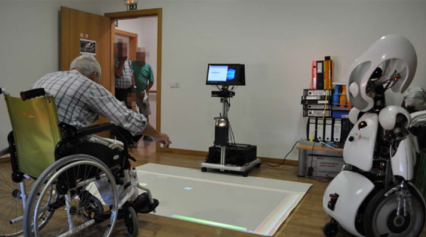
\includegraphics[width=0.8\linewidth]{images/old.png}
      \caption{Elderly Care Facility}
    \end{subfigure}%
    \begin{subfigure}{.5\textwidth}
      \centering
      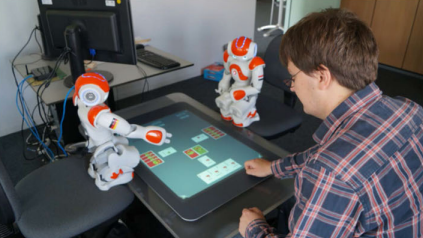
\includegraphics[width=0.8\linewidth]{images/multiple.png}
      \caption{One Human and Multiple Robots playing}
    \end{subfigure} 
    \caption{Interactions human-robot}
    \label{fig:interactions}
\end{figure}

\subsection{Reasoning Agents}
Rush Hour has been the subject of various studies in the field of artificial intelligence, particularly in the area of planning. It has been a popular test-bed for artificial intelligence research since its inception in the late 1990s since the game presents an interesting challenge for AI systems due to its complex and dynamic nature, which requires the system to reason about how to move vehicles on a crowded grid to reach a target location. Over the years, researchers have applied a variety of AI techniques to solve the Rush Hour puzzle, including search algorithms, constraint satisfaction, planning, and even neural networks. Researchers have developed a variety of planning algorithms for the Rush Hour game, including real-time heuristic search, PDDL-based planning, and constraint satisfaction algorithms. In \cite{minizinc} the authors provide a constraint programming encoding in MiniZinc and a model in Answer Set Programming for the game. In \cite{genetic} they evolve heuristics to guide IDA* search for the 6x6 and 8x8 versions of the Rush Hour puzzle: starting from several novel heuristic measures the authors turn to genetic programming (GP).\\
\indent In our case, we decide to use AIPlan4EU (\url{https://www.aiplan4eu-project.eu/}) which allows us to access existing planning technologies.  


%* solution: architecture of the solution, possibly with a figure showing which components have been developed within the project, which already existing components have been used and integrated, how they are connected to each other, etc. In particular, highlight the HRI and the RA parts. Contributions of both HRI and RA must be explicitly stated.
\section{Solution}

\begin{figure}[H]
    \centering
    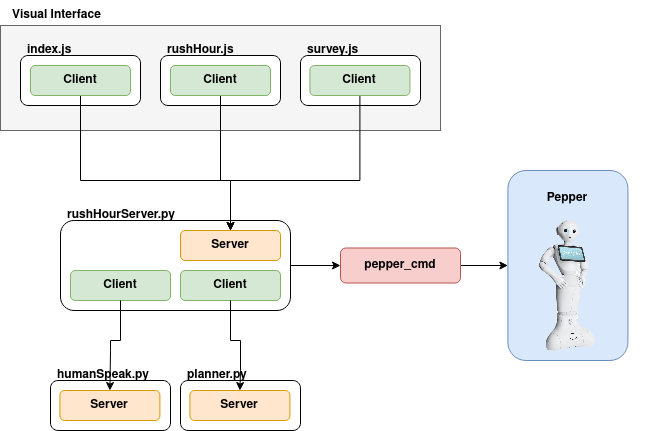
\includegraphics[width=\textwidth]{images/architecture.drawio.png}
    \caption{Proposed architecture.}
    \label{fig:architecture}
\end{figure}

The architecture of the proposed solution is displayed in \ref{fig:architecture}. The core of the structure is the main server (\textit{rushHourServer.py}), which is used as a crossroads that puts into communication all the different modules of the project and it is written in Python. We chose to put the rushHourServer as a crossing point for every communication because the functions contained in \textit{pepper\_cmd} are only accessible there. So each time a message is received by the server, we can trigger a Pepper behavior (motion or speech) relative to the current event. The flow of information follows the following scheme:

\begin{enumerate}
    \item When the interface is set up, a request to determine the state of the game is sent to the main server. We could be in two situations: the interface has been loaded for the first time since a user completed the interaction, or it has been loaded after one instance of the game has been solved. Depending on which situation we are in, the display shows different information.
    \item If the interface loads for the first time, it stays in an idle state until the server sends a message indicating that a human has entered Pepper's area of interaction (less than 1.5m in front of the robot). In this case the interface loads the initial survey and shows it to the user.
    \item Each text shown in the interface is sent to the main server, which triggers an event that results in Pepper saying said text. This way, the user can read or hear the question asked by Pepper.
    \item During this survey, the \textit{humanSpeak} module comes into play. In fact, given has two means to understand the request made by Pepper (hearing or reading), we gave them the ability to interact in both ways, by speaking or pressing buttons on the tablet. Given that we are not using the real robot, but a simulated environment, it's not possible to actually speak to the robot, but to simulate this, the \textit{humanSpeak} module features a console that prompts the user to write what they would like to say to the robot. The user is able to choose between a fixed set of words, that the robot is programmed to understand, which correspond to the text visible on the buttons they are able to press on the interface. This data relative to the current question is sent to a server hosted in the module, which displays it in the console, and waits for a response by the user. They have 10 seconds to say something. If they don´t say anything, we assume they want to interact with the robot via the tablet. If they do say something (i.e. write it in the console), the message is sent to the main server, which forwards it to the interface, prompting a change of scene. The behavior is exactly the same as that obtained when pressing the corresponding button. The mean of communication with Pepper can be chosen freely at each moment, independently from what the user chose in previous instances. 
    \item At the end of the survey, the interface sends the temporary result to the main server, which stores them in the main server, waiting for the additional results produced in the final survey after the match. The game interface is loaded.
    \item As the game interface appears, a request for the data relative to the chosen level is sent to the server, which responds with the desired configuration of the board. At this moment, the user can start playing.
    \item After each move, a message is sent to the main server, containing the updated configuration of the board. The server forwards this information to the other server module in our architecture, the \textit{planner}. It receives the data about the board configuration from the main server, and computes the desired plan for the solution of the game. From this plan, we extract just the first move, and we return it to the visual interface, which updates the board accordingly. After this move performed by Pepper (to which a coherent animation of the robot corresponds), the turn passes again to the user, and the cycle repeats.
    \item The game ends when Pepper, or the user, make a move that brings the red car in the goal position. At this point the interface changes again, showing a screen where the user is asked whether they want to play another match, or start a survey regarding their experience.
    \item In the first case the user is brought to the choosing level screen, while in the other scenario the interface changes, showing the survey.
    \item When the survey loads, a request is made to the main server, which responds with the object containing answers the same user gave during the initial survey, which is then updated with the answers given in this final survey, and sent again to the server.
    \item This marks the end of the interaction with the robot, which goes to the initial state, waiting for a human to approach it.
\end{enumerate}

The diagram visualizing this interaction flow is shown in \ref{fig:flow}, and described in more detail below, with less focus on the technical implementation, and more details regarding the Human-Robot Interaction.

%QUESTA PARTE QUI SOTTO SECONDO ME SI PUÒ TOGLIERE
\begin{comment}
The interaction between Pepper and the user is subdivided into several phases:
\begin{enumerate}
  \item The initial phase where Pepper waits for a human and when someone is closer to him, Pepper presents himself and asks some questions e.g. the username of the player, if the player is a novice, if the player wants the rules of Rush Hour;
  \item The second phase if the match played in a collaborative way between human and robot so here we have the reasoning component but also a part of HRI since here the robot will perform some animations;
  \item The third and final phase is made of other questions from Pepper such as if the player wants to play another match, if the player will suggest the robot to a friend of him and if the experience has been good.
\end{enumerate}
\begin{enumerate}
  \item Initially Pepper waits in an idle state for a human to approach it. Its display shows the text "Waiting for someone to play with me...", inviting people to come closer to it. Once a person gets to a distance less than 1.5 meters, Pepper detects them with its frontal sonar and starts the interaction.
  \item The second phase is a short survey in which Pepper acquires some information about the potential player
\end{enumerate}
All of these information will be stored in order to profile the users of the social robot.
\end{comment}
\subsection{Human-Robot Interaction}
\begin{figure}[H]
    \centering
    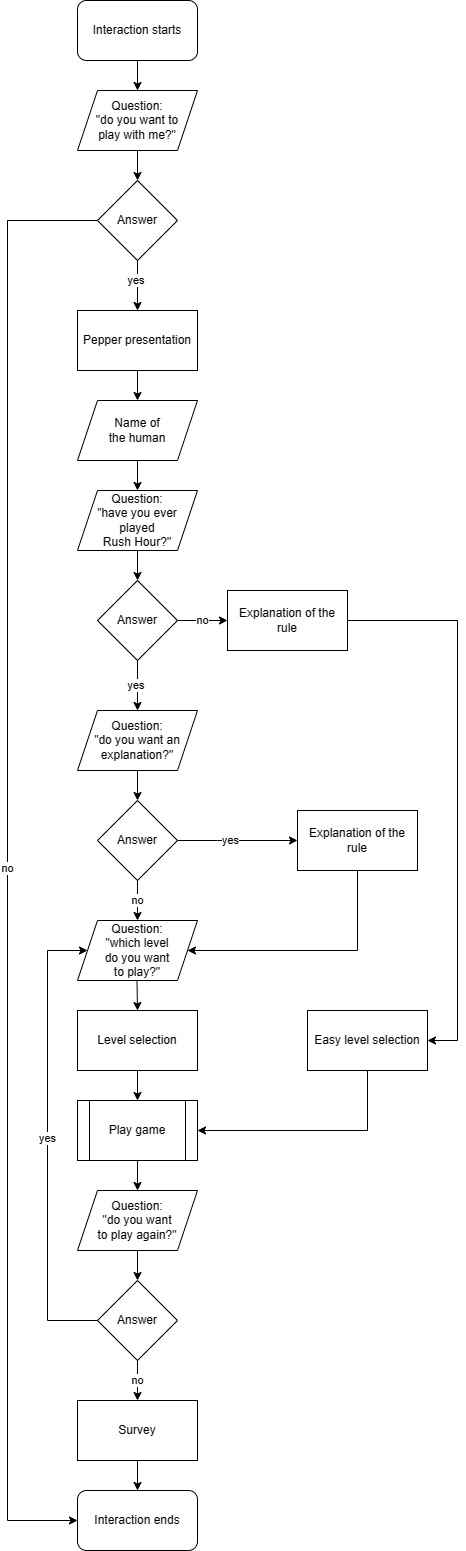
\includegraphics[width=.36\textwidth]{images/flow_diagram.png}
    \caption{Flow diagram of the HRI part.}
    \label{fig:flow}
\end{figure}
\indent The flow diagram concerning Human-Pepper interaction is shown in Figure \ref{fig:flow}. Initially Pepper waits in an idle state for a human to approach it. Its display shows the text "Waiting for someone to play with me...", inviting people to come closer to it. Once a person gets to a distance less than 1.5 meters, Pepper detects them with its frontal sonar and starts the interaction. To be clear and immediately state its intentions, Pepper asks the human whether they want to play a match of Rush Hour game with him; the human may accept, or refuse. In the latter case, Pepper communicates its displeasure to the user and after some seconds re-display the initial page, waiting for another user to connect with. If the user accepts, on the other hand, Pepper starts a small survey, which will be stored in the server, regarding the user and past experiences with the game. It will prompt the user for a username, which will be used to store their data, and whether they have already played the game, or need to be reminded the rules. If from this information, the fact that the user doesn't have experience with the game emerges, then Pepper automatically chooses to let the user play the easiest level available. Otherwise, the choice of the difficulty level is left to the human agent.
\\
\noindent After this small survey, the second phase starts, with the human and the robot playing the game in a collaborative fashion. During the game, the two players in turn make their move until the goal is reached, at which point the game ends.\\
\noindent In the third and final phase, Pepper asks whether the user wants to play again or whether it wants to end the interaction, inviting the person to fill another short survey regarding their experience with the game and the robot. The answers to these questions will be joined with those obtained in the first phase and stored in the server. On the other hand, if the user is up to play another match, the interface leads them to the level choice screen, in which the user is able to choose which level they want to play next. To help the user choose wisely, Pepper suggests to play a difficulty level slightly higher than that just played by the user, hoping to make the user face a bigger and more compelling challenge.



%\begin{figure}[H]
    %\centering
    %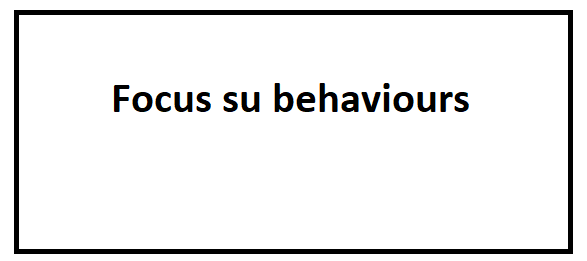
\includegraphics[width=\textwidth]{images/segnaposto_4.png}
    %\caption{Caption of the figure.}
    %\label{fig:segnaposto4}
%\end{figure}

Concerning the Pepper gestural communication, in the images below it's possible to notice when and how four different animations are realized. 

\begin{figure}[H]
    \centering
    \begin{subfigure}{.5\textwidth}
      \centering
      \frame{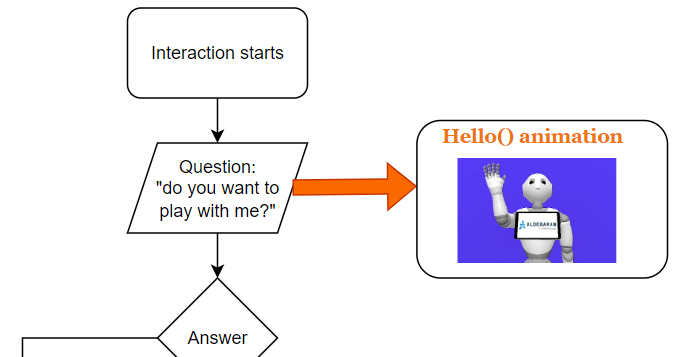
\includegraphics[width=0.9\linewidth]{images/animation_hello.png}} 
      \caption{When and how Pepper hello animation occurs.}
    \end{subfigure}%
    \begin{subfigure}{.5\textwidth}
      \centering
      \frame{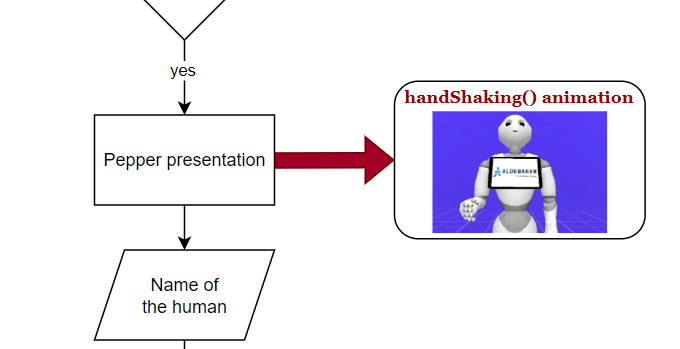
\includegraphics[width=0.9\linewidth]{images/animation_handshaking.png}}
      \caption{When and how Pepper hand shaking animation occurs.}
    \end{subfigure} 
    \begin{subfigure}{.5\textwidth}
      \centering
      \frame{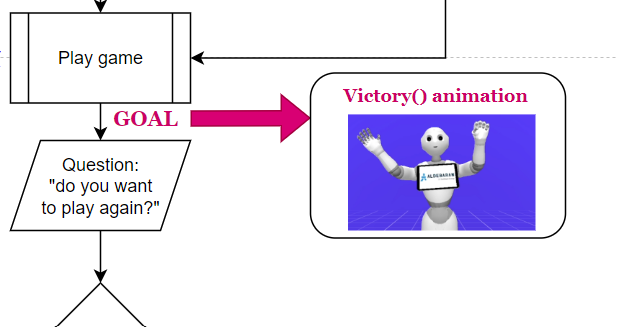
\includegraphics[width=0.9\linewidth]{images/animation_victory.png}} 
      \caption{When and how Pepper victory animation occurs.}
    \end{subfigure}%
    \begin{subfigure}{.5\textwidth}
      \centering
      \frame{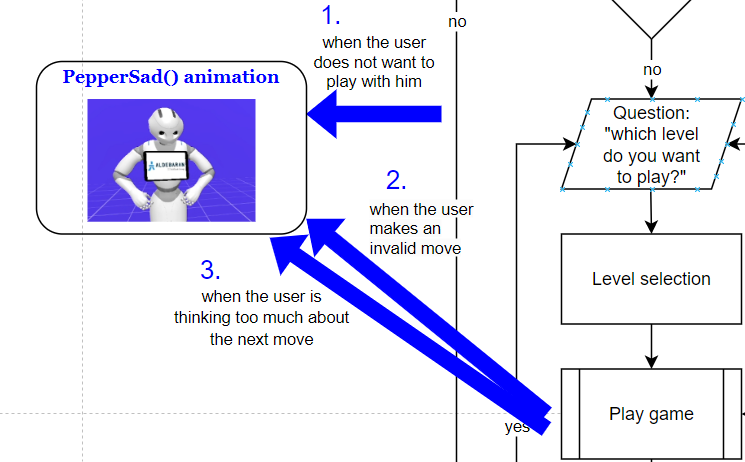
\includegraphics[width=0.9\linewidth]{images/animation_peppersad.png}}
      \caption{When and how Pepper sad animation occurs.}
    \end{subfigure} 
    \caption{Examples of four different Pepper animations.}
    \label{fig:animations}
\end{figure}


Aside from these animations represented in Figure \ref{fig:animations}, we created four additional animations that the Robot execute whenever he makes a move in a certain direction (for details see in the next section).\\
\noindent The reason why the robot gestural communication is fundamental is that it enhances the acceptability aspect of the human toward the robot. In fact, we tried to make the robot's moves as natural as possible in order to improve in the human the sense of confidence and familiarity against the robot, thing that is very important in a lot of social contexts like the medical and the educational one, when the robot has to deal with children and elderly people.


\subsection{Reasoning Agents}
Concerning the reasoning part, as we have already told, in Rush Hour vehicles can only move vertical or horizontal and in particular each vehicle can move forward or backward. In order to implement all of this, first of all we have set a convention of how the vehicle configuration is passed: the first cell is always the "head" of the machine. If the vehicle is towards right, the forward will consist in moving towards right and the backward will consist in moving to left; if the vehicle is towards up, the forward will consist in moving towards up and the backward will consist in moving towards down (see figures \ref{fig:horizontal} and \ref{fig:vertical}) [for vehicles looking left/down the logic is specular].\\
\indent The red car is always instantiated as an horizontal car looking to right and so the goal of the planning problem is reached when its head is at the rightmost cell of the same row. \\
\indent To set the initial configuration of the planning problem, we will pass two arrays: the former contains all the cars and their position on the board (the red car is always the first one of this list), the latter is the list of all the trucks and their positions. For each car we need \textbf{\textit{(id, cell1\_row, cell1\_col, cell2\_row, cell2\_col)}}; for each truck we will need \textbf{\textit{(id, cell1\_row, cell1\_col, cell2\_row, cell2\_col, cell3\_row, cell3\_col)}}. The id is a progressive number representing the vehicle in the board and in this way we always know which car/truck moves.\\
\indent As previously said, we resolve the reasoning aspect using AIPlan4EU and in particular we will return a sequence of actions where each action is one-cell movement of a vehicle. We will give to the HTML the id of the vehicle, the motion type i.e. forward or backward and how many cells the vehicle moves.

\begin{figure}[H]
    \centering
    \begin{subfigure}{.5\textwidth}
      \centering
      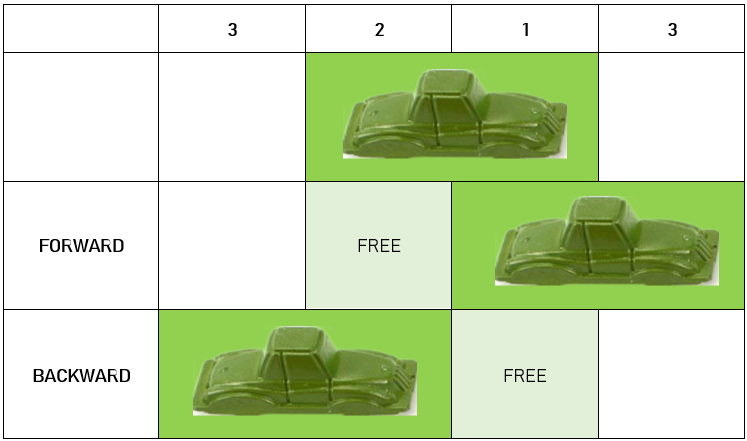
\includegraphics[width=.82\linewidth]{images/hor_car.png}
      \caption{Moves for horizontal cars}
    \end{subfigure}%
    \begin{subfigure}{.5\textwidth}
      \centering
      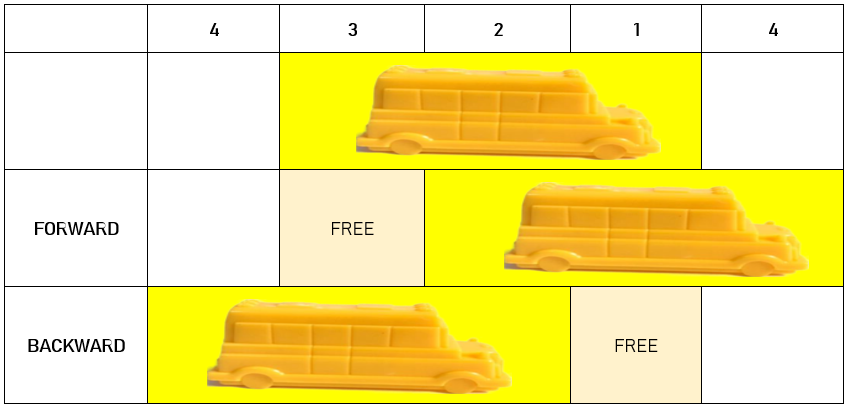
\includegraphics[width=1\linewidth]{images/truck_or.png}
      \caption{Moves for horizontal trucks}
    \end{subfigure}
    \caption{Moves for horizontal vehicles}
    \label{fig:horizontal}
\end{figure}
\begin{figure}[H]
    \centering
    \begin{subfigure}{.5\textwidth}
      \centering
      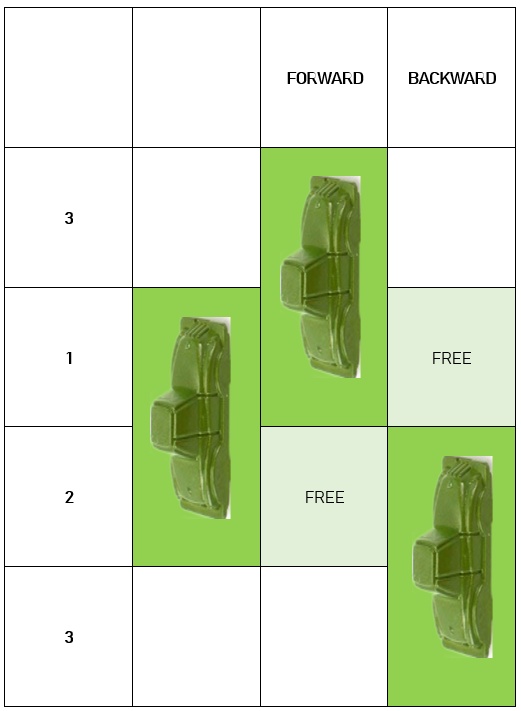
\includegraphics[width=\linewidth]{images/ver_car.png}
      \caption{Moves for vertical cars}
    \end{subfigure}%
    \begin{subfigure}{.5\textwidth}
      \centering
      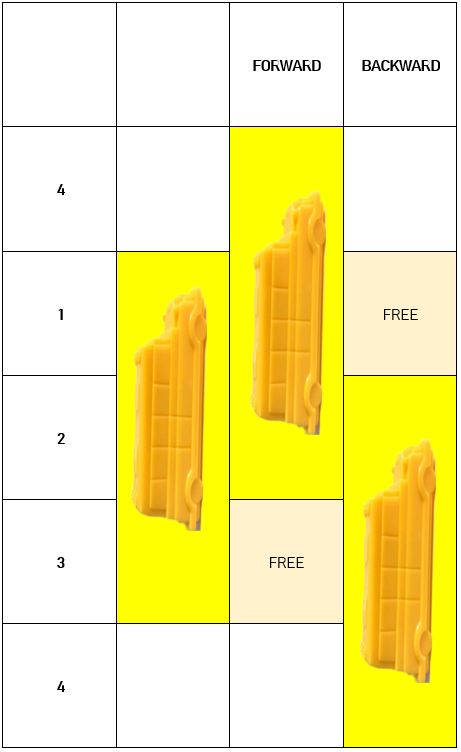
\includegraphics[width=0.83\linewidth]{images/truck_ver.png}
      \caption{Moves for vertical trucks}
    \end{subfigure}
    \caption{Moves for vertical vehicles}
    \label{fig:vertical}
\end{figure}


%* implementation (details on the implementation, which libraries/tools you have used to implement the components, how do you put them all together). Again, explicit descriptions for both HRI and RA is required.
\section{Implementation}
\noindent This section provides a detailed explanation of how each component of the project has been implemented, from the tools and frameworks that have been used to the reasons motivating our choices.

\subsection{Experimental setup}
%\noindent This project has been developed in a Linux environment, in particular using Docker, which allows creating a container where it is possible to work independently from the rest of the system. In this way, any change made on or by the code toward Pepper's environment or framework are not permanently applied, therefore it is not affected by development problems. This capability is provided by an additional abstraction through OS-level virtualization by executing the following commands: i) run a docker image with all libraries considered:
%\lstinputlisting[language=Octave, firstline=1, lastline=1]{codes/dockerCode.txt}
%and run such image to enter the architecture of your robot:
%\lstinputlisting[language=Octave, firstline=2, lastline=2]{codes/dockerCode.txt}

%\begin{wrapfigure}{r}{0.5\textwidth}
%    \begin{center}
%        \includegraphics[width=0.8\linewidth]{images/naoqi_architecture.png}
%    \end{center}
%    \caption{NAOqi architecture.}
%    \label{fig:naoqi_architecture}
%\end{wrapfigure}

%\noindent With these commands it is possible to create various environments in which to start a NAOqi server for virtual or physical connection to a Pepper robot and other environments for the execution of additional functionalities. For example, one of such environments has been used to activate a server that could connect together Pepper, the graphical website for user interaction, and the planner for providing intelligent responses to the game by the robot. Similarly, a separate environment is needed for using the NAOqi server, to allow the communication with the robot, which is located at the top of the hierarchy of the architecture which it is a part of. This hierarchy is shown in figure \ref{fig:naoqi_architecture}.\\
The project has been developed fully in a Linux environment. For the installation of the tools used to communicate with the robot Pepper we used a docker image with all the packages and programs necessary to do so. 

Given that we didn't have the physical robot at our disposal, we had to rely on a simulated version of Pepper. We opted to simulate it in Choregraphe, an application developed by Aldebaran Robotics, which is very useful to design and develop animations, behaviors and dialog for robots, and test them in simulated environments.

To write the functions of the modules that compose our architecture (see Figure \ref{fig:architecture}), we decided to use Javascript, HTML and CSS for the components that make up the visual interface displayed in Pepper's tablet, while we used Python for the programs that manage the definition and solution of the planning problem, and for the development of the main server, that manages all the communications between the different components of the project.

To exchange data between these components, we made use of WebSockets. Javascript natively supports these means of communication, so we didn't have to use any external library, while for Python programs, we decided to use Tornado, a framework used to create and manage scalable web servers in Python.

\subsection{Human-Robot Interactions}
\subsubsection{Use of \textit{Pepper\_tools} modules for Pepper communication}

The process that sees Pepper involved in the interaction with the human happens through a python program in which we make use of \textit{pepper\_tools} utilities. \textit{pepper\_tools} is a repository that contains different tools to manage the Softbank Pepper robot. As we can see from image shown in figure \ref{fig:detail_of_pepper_tools}, there are multiple modules in pepper\_tools that make Pepper perform different tasks: using its sensors, making some physical moves, managing audio inputs and outputs  or saying something.

\begin{figure}[H]
    \centering
    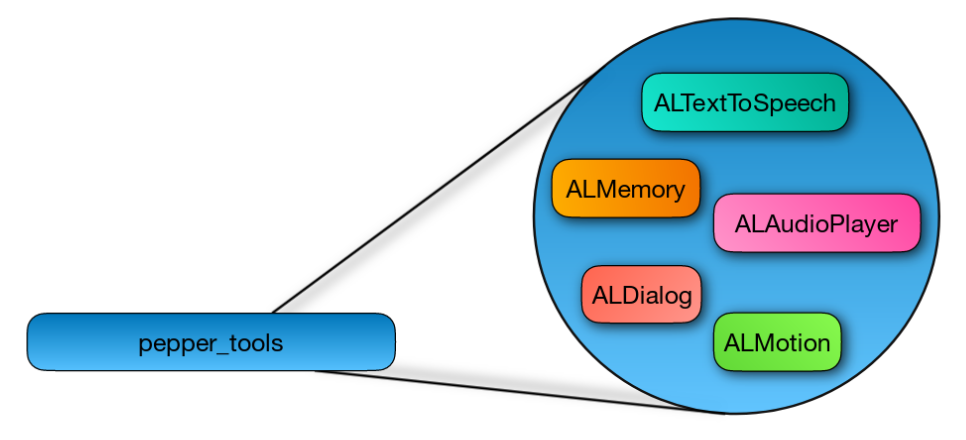
\includegraphics[width=0.6\textwidth]{images/detail_of_pepper_tools.png}
    \caption{Modules in \textit{pepper\_tools}.}
    \label{fig:detail_of_pepper_tools}
\end{figure}

\noindent First of all, once we establish the connection with the simulated robot, we make use of some \textit{pepper\_tools} functions to read the information provided by the virtual sonar sensor. Whenever the distance of the user from the robot is less  than a meter and a half, the interaction begins. Actually, since we work with simulated Pepper we made sure that, whenever we say that we “enter scene”, the distance from the robot is 1,20 meters: from this moment the interaction starts.

\lstinputlisting[language=Python, firstline=21, lastline=32]{codes/sonar.py}

%!!!!!!! nel codice non c'è la chiamata esplicita a ALTextToSpeech !!
\noindent Then, in order to make the robot speak, the ALTextToSpeech module is used. In particular, ALTextToSpeech sends the sentence that the robot has to say to a text-to-speech engine and the result of this synthesis is sent to the robot. The module also endorses voice customization, such as speed or language. This module is used through the call of the function \textit{say} that is utilized whenever, during the interaction, the robot starts saying something to the human. Actually, since we use the simulated robot, we will know that Pepper on Choregraphe is saying something by seeing a dialogue box above him. In the image below, an example of how the function is called is shown. 

\lstinputlisting[language=Python, firstline=177, lastline=185]{codes/rushHourserver.py}

\noindent Another use of \textit{pepper\_tools} modules that makes the robot move is the ALMotion module. We developed 8 python customized functions that make the robot do some animations during the interaction, starting from the the initials “Hello” and “Hand Shaking”  motions that the robot make to greet the human, to the movements that the robot make to shift a car or a truck during its move in the game, to the final Pepper reaction if the game ends in a victory. All the functions are manually implemented and each of these present different timelines. Above it’s showed the “Hand Shaking” function that is executed by the robot in the initial presentation phase, after the “Hello” motion, in order to introduce itself to the human. 

\lstinputlisting[language=Python, firstline=85, lastline=110]{codes/pepperAnimations.py}

Other examples of animation are the four possible moves that the robot can make during the game: moving a car or truck horizontally on the right or on the left or moving a car or truck vertically up or down; the code of the “MoveVerticalUp” animation is specified above in figure *. 

\lstinputlisting[language=Python, firstline=160, lastline=181]{codes/pepperAnimations.py}

Finally, we implemented two additional animations: the first, “PepperVictory”,  is called when the human and Pepper win the game and the second, “PepperSad”, is called (in three different situations) when the user decides to not play the game with him, when the user is thinking too much about the next move to make and when the user makes an invalid move. 

\lstinputlisting[language=Python, firstline=33, lastline=58]{codes/pepperAnimations.py}






%----------------------------SOF------------------------------------------
\noindent As we will better explain in the following, the robot suggests a level to the user by performing some simple reasoning over the received answers. After the questionnaire, the user can select the level he wants and start playing. In order to collaboratively solve the game, the user and the robot need to execute a move alternately. While doing so, the robot informs the user when it is its turn to play and mimics to the user the direction in which Pepper has decided to move the object. This movement is implemented through a custom function similar to \textit{doHello()}.
While playing, Pepper also warns the user when he tries to make an invalid move, such as picking from an empty rod or trying to move a disk on a smaller one. This is done by receiving messages from the web application through a websocket, as will be better explained in one of the following sections. The warning is given to the user by using the aforementioned \textit{asay}, whose name stands for animated say, meaning that the robot gesticulates while speaking.

\lstinputlisting[language=Python, firstline=52, lastline=62]{codes/clientPepper.py}

\noindent Finally, when the robot and the user manage to win by moving all the disks to the rod on the right, the robot informs the user while making a little victory dance, that has been implemented similarly to the \textit{doHello} function, leveraging the ALMotion module. The robot then invites the user to rate his experience and the difficulty he encountered using the tablet, as we will better explain later, and he can then play again or leave.

\subsubsection{Website for interaction through the tablet}
During its period of activity, Pepper keeps showing a visual interface on its tablet. This interface is developed using the standard technologies that are commonly used when developing applications that run on a browser: HTML, CSS and Javascript. We subdivided the interface in three different sections, each one composed by a triplet of files, one for each of the aforementioned technologies. The HTML files simply describes the structure of the page, and they are all fairly straightforward. As an example, below is the body of the HTML file for the game interface (\textit{rushHour.html}).

\lstinputlisting[language=HTML, firstline=11, lastline=33]{codes/rushHour.html}

The corresponding CSS file is simply used to style all the elements of the page, to make it more visually pleasing, but adds no functionality.

All of the logic of the page is implemented in the Javascript file \textit{rushHour.js}. Here we have two classes defined: 
\begin{enumerate}
    \item A Board class, representing the area in which the game takes place, initialized once each time the page is loaded. The most important field of this class is \textit{status}, a 2D matrix made of arrays of arrays which keeps an updated status of all the cells in the board. If a cell is occupied by a vehicle, the corresponding cell in the array contains the id of the vehicle. It also has some helper methods used to set it up when the game begins, to check whether the current configuration corresponds to a win (and thus end the game), or export the state of the board to send it to the planner, which will return the next move made by Pepper.
    \item A Piece class, representing one vehicle of the game. Each piece has an \textit{id} to uniquely identify it, (the car the player has to move always has id=1), and some defining properties such as \textit{color}, \textit{orientation} (vertical or horizontal), \textit{length} (which can be equal to 2 or 3, depending if the piece represents a car or a truck), and the coordinates in the board of the rightmost cell, in case of horizontal pieces, or the highest cell, in case of vertical pieces. This class too has some methods to manipulate it. The most important one is the \textit{move} method, which is called each time the human or Pepper wants to move a piece of the board. We also used methods such as \textit{reset} and \textit{setBoard} to change the appearance of the board when a piece is moved, and \textit{highlight} and \textit{dehighlight} to change the visuals of the piece to let the player know when they selected it.
\end{enumerate}

This page also features some buttons similar to the arrow keys present on every keyboard, to let the user easily move each piece on the board.

When this page first loads, a WebSocket to the main server is opened. A request to the server is made, asking for the initial configuration of the board. The server responds choosing a level based on the user's answers in the initial survey. After this, the socket is kept open, and a message is sent to the server each time the user makes a move. This message contains the updated configuration of the board. The server forwards this request to the planner, which computes a plan to let the car out of the board, and sends the first move of this plan to the server, which in turn forwards it to the interface, which finally displays Pepper's move.

Other than this, if too much time passes since the last message arrived to the interface (i.e. since Pepper made its last move), a message is sent to the server, which makes Pepper ask the user if they are having difficulties find the next move.

Below is the implementation of this socket

\lstinputlisting[language=C, firstline=276, lastline=329]{codes/rushHour.js}

The structure of the initial survey is defined in the file called \textit{index.HTML}. Here too, the main structure is very simple. The main logic is implemented in \textit{index.js}. This file manages all the logic that regulate which scene to display when each button of the survey is pressed, following the flow diagram represented in Figure \ref{fig:flow}. To do so, we implemented a function called \textit{changeScene}, which takes as input an object describing the content of the scene to display, and manages the transition between scenes. First, the text of the scene is displayed with an animation that emulates a person writing in the terminal, that happens at the same time as Peppers says it out loud. It should act as if it were subtitles to what Pepper is saying. After the text is fully displayed and Pepper as said all he had to say, the buttons corresponding to the possible answers of the user appear. When a user presses them, the \textit{changeScene} function is called once again, now passing another object relative to the corresponding scene to be displayed, and the cycle continues, until the press of a button triggers the start of the game, in which case the interface starts displaying the game screen defined in \textit{rushHour.HTML}.

Below is the definition of one of the objects that define a scene. Notice that the object contains information about the text to display, the text in the buttons and their color, and the functions to be called when these buttons are pressed.

\lstinputlisting[language=C, firstline=246, lastline=260]{codes/index.js}

This file too contains a WebSocket that sends information to the main server. This happens when the user selects a the level to play, to communicate it to the server so that it can respond with the correct board configuration when the game starts, and immediately before the game interface is displayed, to send the results of the survey to the server, so that they can be recovered and updated with new information in the final survey at the end of the game.

The aforementioned final survey is described in the file, the file \textit{survey.HTML}. The page is very simple, it contains two rows of radio buttons to let the user answer the asked questions with a rating from 1 to 5. A soon as the page loads, a WebSocket sends a request to the main server for the results that were given in the first survey, which are updated with the new answers of the users, and sent to the server once again when the window is closed and the user interaction ends. An image of this screen is shown in Figure \ref{fig:fourth}.e.



%-------------------------------------------------------------------------------

\subsection{Reasoning Agents}

\subsubsection{Use of AIPlan4EU to plan a solution of the game}
Pepper's reasoning capabilities are provided and implemented through the AIPlan4EU Unified Planning framework which exploits the Unified Planning library. It allows us to solve the problem by the invocation of different automated planner i.e. \textit{pyperplan}, \textit{tamer}, \textit{enhsp}, \textit{fast-downward} and also with the possibility to use heuristics: the usage of several planners is possible thanks to the planner-independent formulation of the planning problem.\\
\indent In the case of the first level
\lstinputlisting[language=Python]{codes/livello_1.py}
the problem will have the following resulting formulation:
\lstinputlisting[language=Python]{codes/problem.txt}
\indent We have declared two types of objects: \textit{cell} and \textit{vehicle}. Cells are always 36 (the board is 6x6) and the number of vehicles changes depending on the level: 9 vehicles in the first level (8 cars + 1 truck),  8 vehicles in the second level (6 cars + 2 trucks) and 5 in the third level (3 cars + 2 trucks).\\
\indent Fluents are variables of the planning problem and they are quantities that can change over time. In our problem definition, we have:
\begin{itemize}
    \item  \textit{free\_cell(x)} which checks if the cell \textit{x} is free or occupied;
    \item  \textit{is\_car(x)} which checks if the vehicle \textit{x} is a car;
    \item  \textit{is\_truck(x)} which checks if the vehicle \textit{x} is a truck;
    \item  \textit{car\_at(x,y,z)} which checks if the car \textit{x} is occupying the cells \textit{y} and \textit{z};
    \item  \textit{truck\_at(x,y,z,w)} which checks if the truck \textit{x} is occupying the cells \textit{y}, \textit{z} and \textit{w};
    \item  \textit{adj\_3(x,y,z)} which checks if the three cells \textit{x}, \textit{y} and \textit{z} are adjacent horizontally or vertically.
\end{itemize}
Note that the adjacency of the four cells in the case of the truck is checked with an AND of two \textit{adj\_3(x,y,z)}.\\
\indent In order to describe the possible evolutions of the system, we declare 4 actions: 
\begin{itemize}
    \item  \textit{move\_forward\_CAR(x,c1,c2,c3)} which allows a car to move forward. In particular cell c3 must be adjacent to cell c1 adjacent to cell c2 (see figure \ref{fig:horizontal} \ref{fig:vertical});
    \item  \textit{move\_backward\_CAR(x,c1,c2,c3)} which allows a car to move backward. in particular cell c1 must be adjacent to cell c2 adjacent to cell c3 (see figures \ref{fig:horizontal} \ref{fig:vertical});
    \item  \textit{move\_forward\_TRUCK(x,c1,c2,c3,c4)} which allows a truck to move forward (the same logic of the car forward motion knowing that a truck occupies three cells);
    \item  \textit{move\_backward\_TRUCK(x,c1,c2,c3,c4)} which allows a truck to move backward (the same logic of the car backward motion knowing that a truck occupies three cells).
\end{itemize}
Each of these four actions is specified through preconditions and effects, defined with fluents.\\
\indent Going on with the explanation, we add all the object of type \textit{Cells} and \textit{Vehicle} to the problem and we initialize the fluents making the "small-world assumption" i.e. it suffices to indicate the fluents that are initially true. The \textit{free\_cell} fluent is initialized starting from the occupied cells that we know from the two set \textit{cars} and \textit{trucks}.\\
\indent We gave a particular attention to the red car for which we save the row and the UP object since we use them to set the goal of the planning problem.\\
\indent As planner, after having tested all the planners offered by the framework, we have decided to use \textit{fast-downward} which will return the optimal path to the goal starting from the given configuration. The problem defined above is passed to this solver, that is called by the program as follows:
\lstinputlisting[language=Python]{codes/planner.py}
\indent Once the planner returns the path i.e. a sequence of actions, we work on it taking only the first actions, all regarding the same vehicle and the same type of motion. To the web browser we send the id of the vehicle, the type of the motion and the number of moves in that direction and in this way the game evolves: the planner will wait for the human to take the next action and then will recompute a new plan given the new configuration.
 
%* results for both HRI and RA functionalities: description of some interactions, possibly commenting portion of the video, showing different modalities of interaction, different behaviors depending on different situations, different reasoning abilities, etc.
\section{Results}
In this section all the distinct parts we presented above merge in a social and reasoning agent and the final result of our project is shown. Initially, the robot waits for a human to come near him using the sonar sensor: when the human gets close to the robot the interaction starts (figure \ref{fig:initial}). The usage of this sensor allows the robot to not invade the human personal space in the case in which the human doesn't want to begin an interaction with the robot. 

At the beginning of the interaction, the connection between the simulated robot and the webpage is established; in this way, we have that the communication between Pepper and the human is instantiated on two channels: through the webpage (with the buttons and the text window) and through the human voice (this last thing is simulated writing on the Ubuntu terminal).\\
\indent After the initial greetings, Pepper asks to the user if he wants to play Rush Hour game with him (fig \ref{fig:first}): if the human refuses, Pepper becomes sad and after 15 seconds returns to check for other humans around him, otherwise Pepper asks to the human his username.

\begin{figure}[H]
    \centering
    \begin{subfigure}{.5\textwidth}
      \centering
      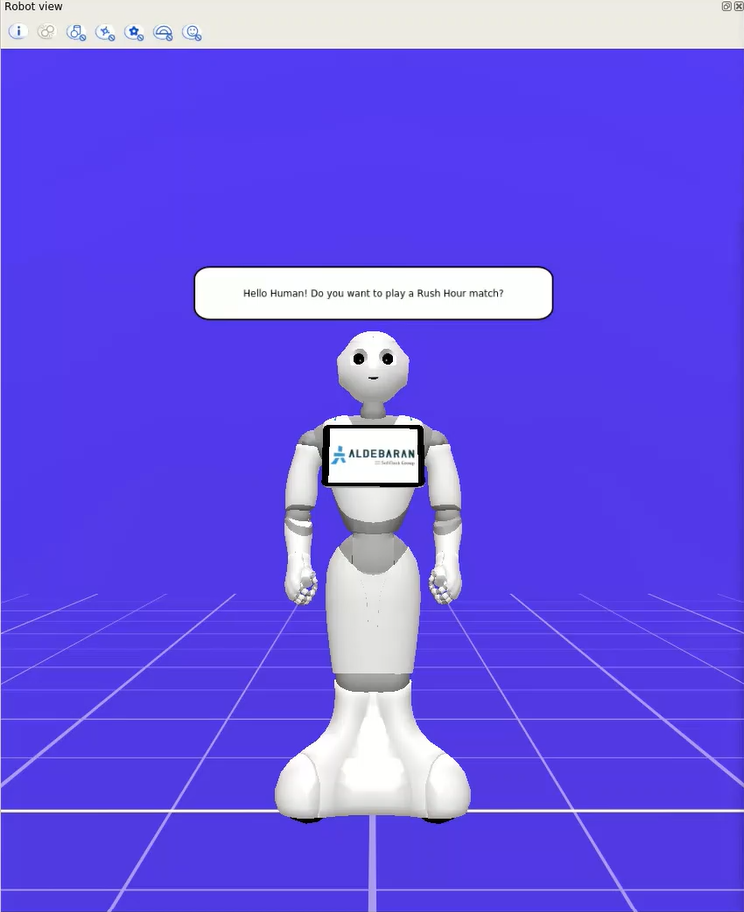
\includegraphics[width=0.9\linewidth]{images/2_umano detectato.png}
      \caption{What Pepper says when a human is detected.}
    \end{subfigure}%
    \begin{subfigure}{.5\textwidth}
      \centering
      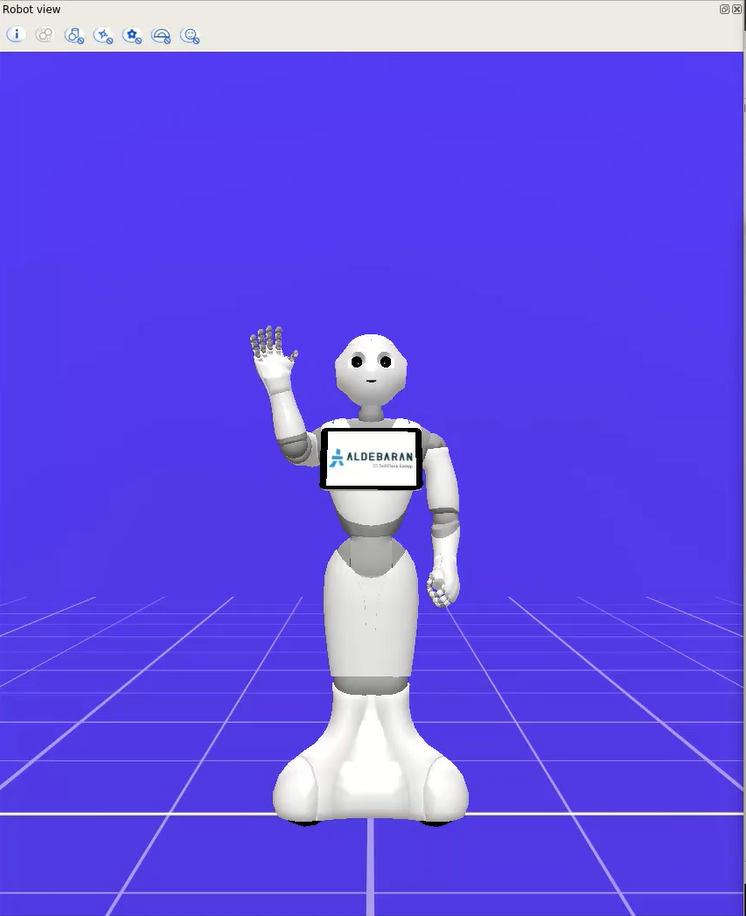
\includegraphics[width=0.9\linewidth]{images/3_ciao umano.png}
      \caption{Hello animation of Pepper.}
    \end{subfigure}
    \caption{Initial greeting of Pepper.}
    \label{fig:initial}
\end{figure}

\begin{figure}[H]
    \centering
    \begin{subfigure}{.33\textwidth}
      \centering
      \frame{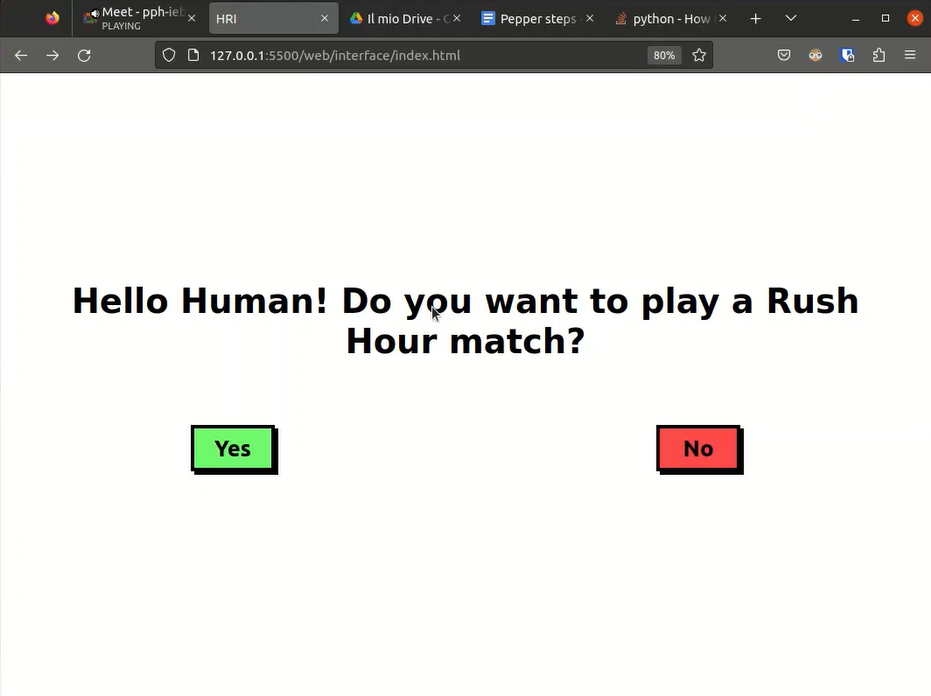
\includegraphics[width=0.9\linewidth]{images/4_vuoi giocare.png}}
      \caption{Match request.}
    \end{subfigure}%
    \begin{subfigure}{.33\textwidth}
      \centering
      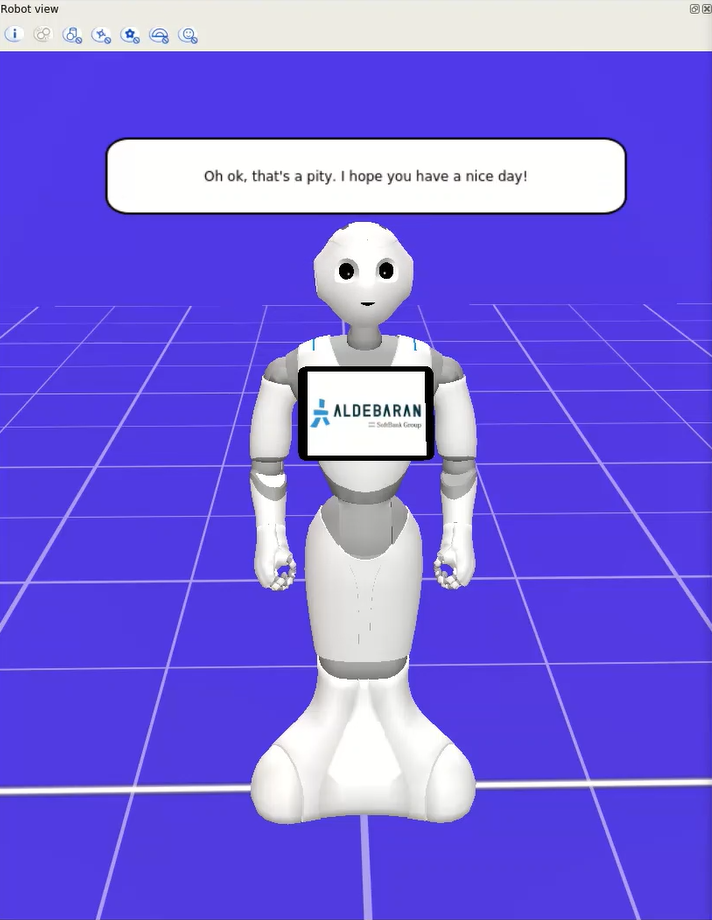
\includegraphics[width=0.9\linewidth]{images/21_non voglio giocare.png}
      \caption{Human's rejection. }
    \end{subfigure}
    \begin{subfigure}{.33\textwidth}
      \centering
      \frame{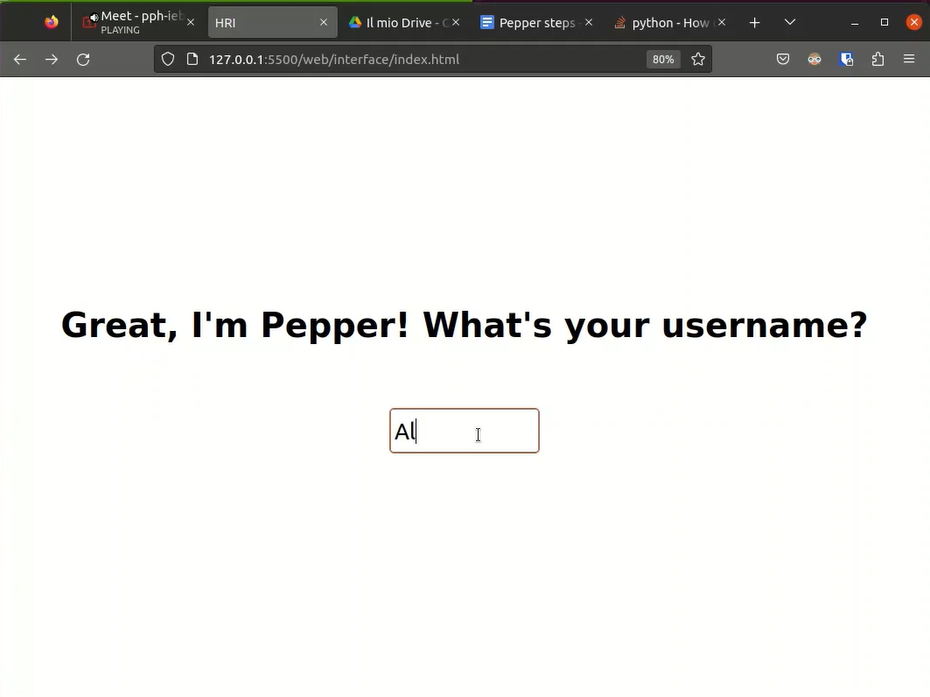
\includegraphics[width=0.9\linewidth]{images/5_inserisci il nome.png}}
      \caption{Asking for the name.}
    \end{subfigure}
    \caption{Reactions to the first questions.}
    \label{fig:first}
\end{figure}

The second question that Pepper asks to the human if he has already played to Rush Hour game and if the answer is "no" Pepper explains the rules and directly selects the easy level instead if the answer is "yes" Pepper asks anyway if the human want to be remembered about the rules. In the latter case, the human will select the level by himself. 

\begin{figure}[H]
    \centering
    \begin{subfigure}{.5\textwidth}
      \centering
      \frame{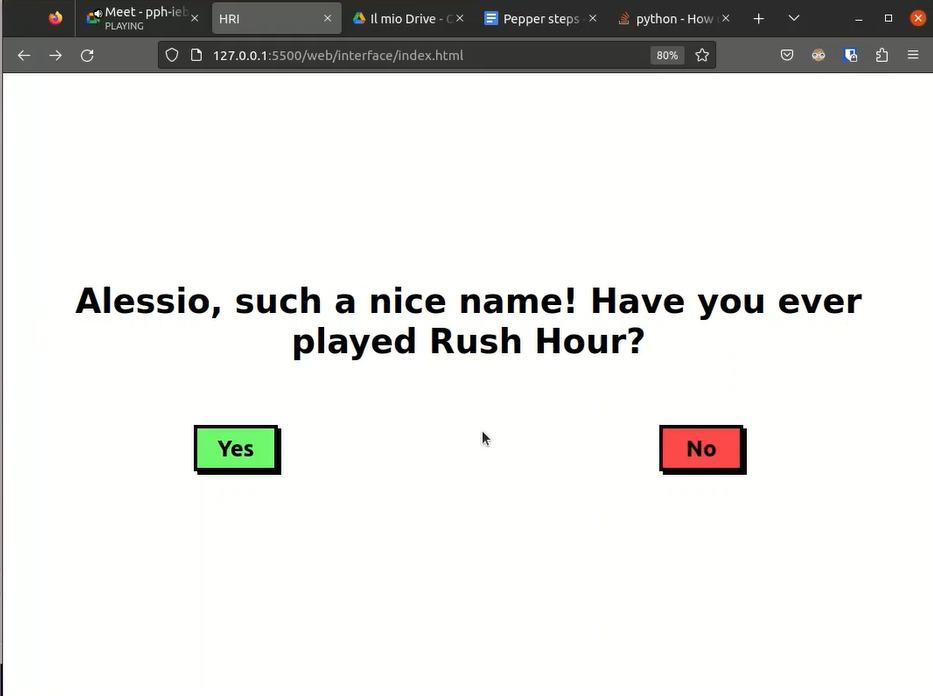
\includegraphics[width=0.7\linewidth]{images/6_hai mai giocato.png}}
      \caption{Experience in Rush Hour game.}
    \end{subfigure}%
    \begin{subfigure}{.5\textwidth}
      \centering
      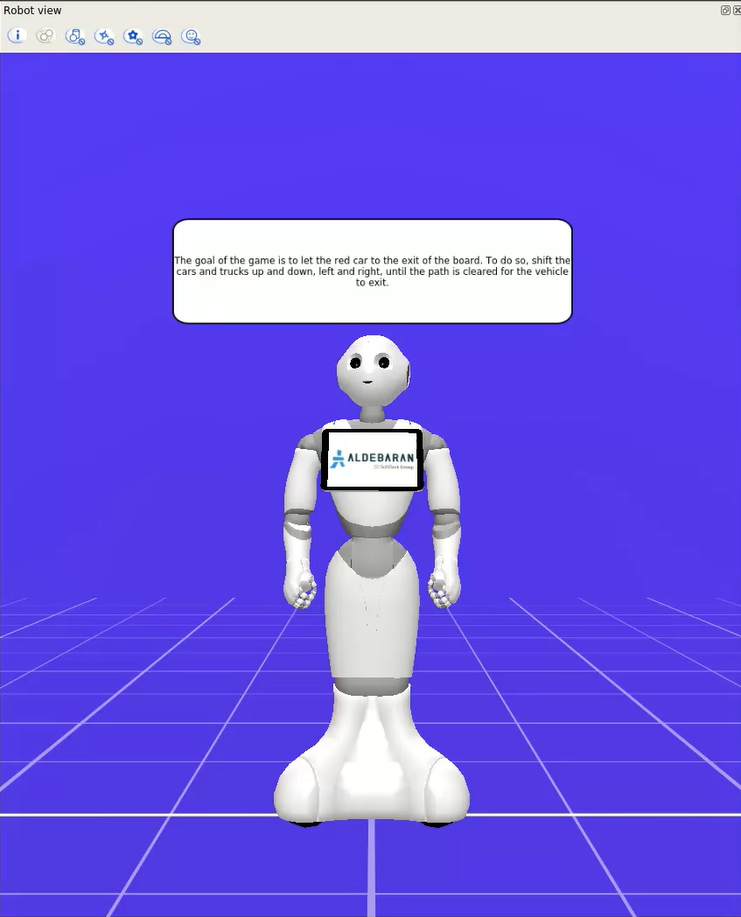
\includegraphics[width=0.7\linewidth]{images/7_pepper spiega le regole.png}
      \caption{Pepper's rules explanation.}
    \end{subfigure}
    \newline
    \begin{subfigure}{.5\textwidth}
      \centering
      \frame{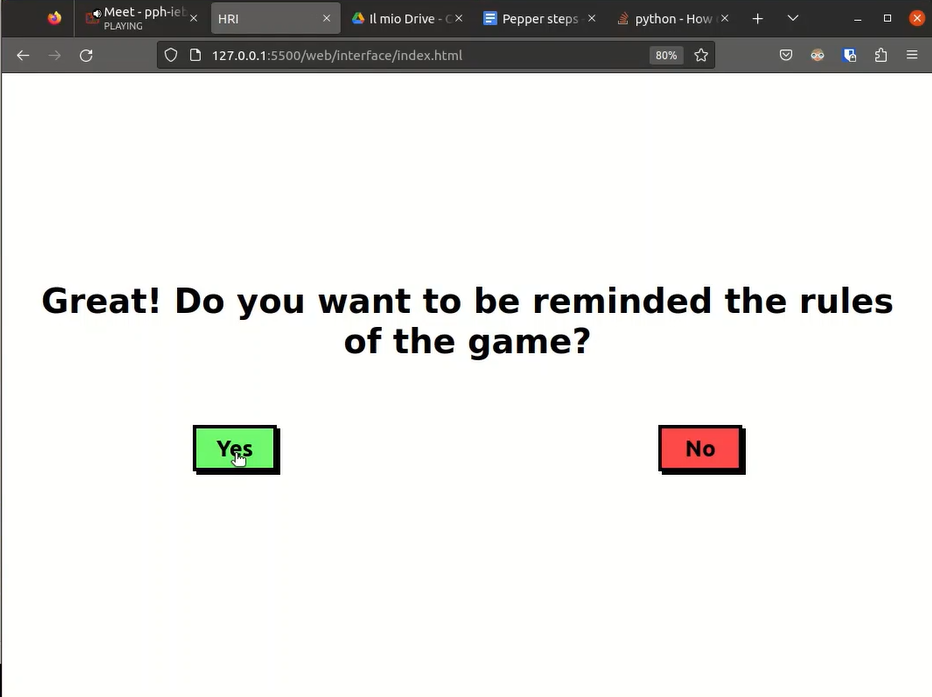
\includegraphics[width=0.7\linewidth]{images/18_giocato ma vuoi lo stesso regole.png}}
      \caption{Rules reminding.}
    \end{subfigure}%
    \begin{subfigure}{.5\textwidth}
      \centering
      \frame{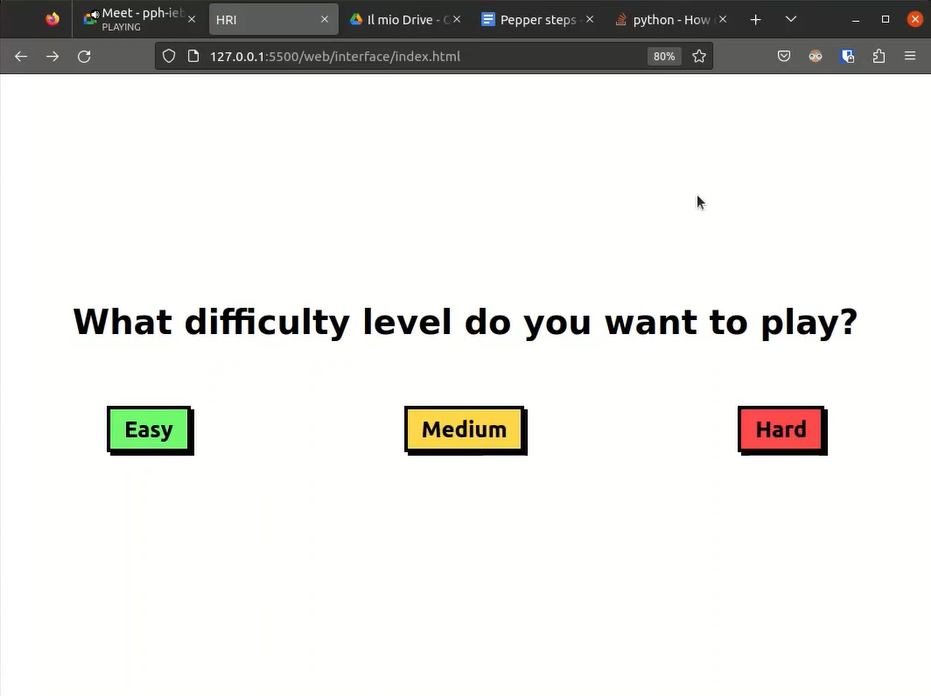
\includegraphics[width=0.7\linewidth]{images/19_seleziona livello.png}}
      \caption{Level selection.}
    \end{subfigure}
    \caption{Rules and level selection.}
    \label{fig:second}
\end{figure}

The human and the robot start playing the game in a collaborative way. Right after the human selects the level for the game, a new connection is opened between the HTML page and the Planner through the main server. The Planner, whenever receives the configuration of the game with the move made by the human, has to send a message to the main server which forwards it to the HTML in which the next move (which represents the robot next move) is specified. On the other side, there is the human which plays the game with the robot using the HTML page. At the same time, there is the robot that, based on the moves computed by the planner, receives some messages about its next moves as they are being forwarded by the main server, in order to perform animations and in order to interact with the human in the correct way. While the match is ongoing, in fact, Pepper speaks to the human and makes animations in different situations (figure \ref{fig:third}): 
\begin{itemize}
    \item when the human performs an invalid move Pepper warns him. An invalid move is when the car or truck is moved outside the board or when is blocked by another vehicle;
    \item when the user is taking too much time to think about the next move, Pepper asks if he is struggling. In particular, Pepper waits 1 minute before posing the question;
    \item when Pepper's turn arrives, he communicates to the human that he's thinking about the next move;
    \item in the first 2 situations listed above, Pepper in the meanwhile performs the animation \textit{PepperSad};
    \item when Pepper plays its move, he shifts his arm simulating the moving vehicle in the specified direction.
\end{itemize}

\begin{figure}[H]
    \centering
    \begin{subfigure}{.33\textwidth}
      \centering
      \frame{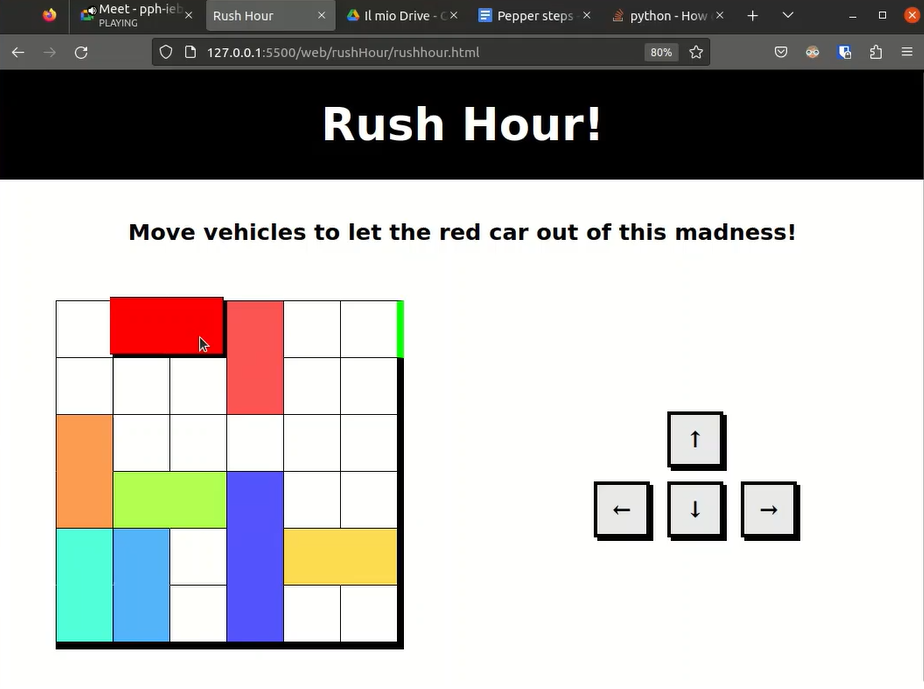
\includegraphics[width=0.9\linewidth]{images/8_uomo gioca.png}}
      \caption{Easy level configuration.}
    \end{subfigure}%
    \begin{subfigure}{.33\textwidth}
      \centering
      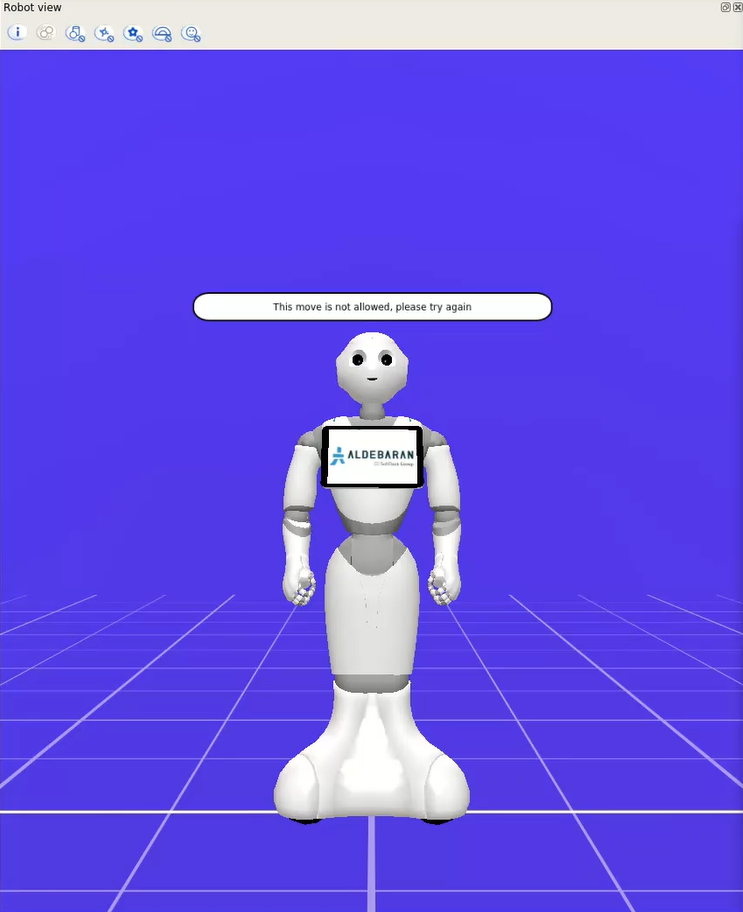
\includegraphics[width=0.9\linewidth]{images/9_mossa invalida.png}
      \caption{Invalid move reaction. }
    \end{subfigure}%
    \begin{subfigure}{.33\textwidth}
      \centering
      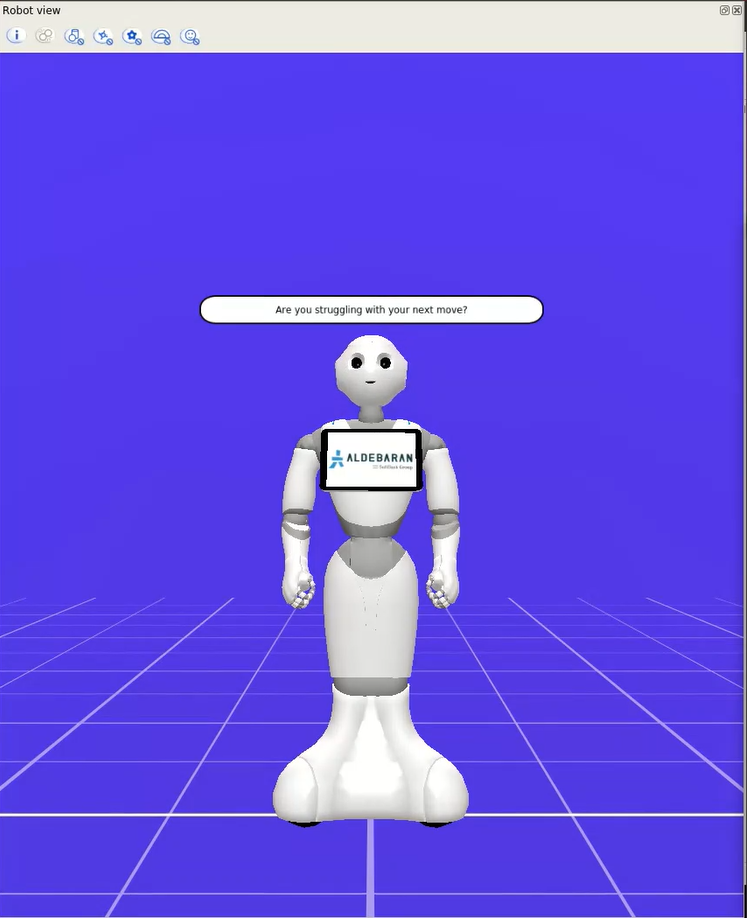
\includegraphics[width=0.9\linewidth]{images/11_troppo tempo.png}
      \caption{Reaction to user struggle.}
    \end{subfigure}
    \newline
    \begin{subfigure}{.33\textwidth}
      \centering
      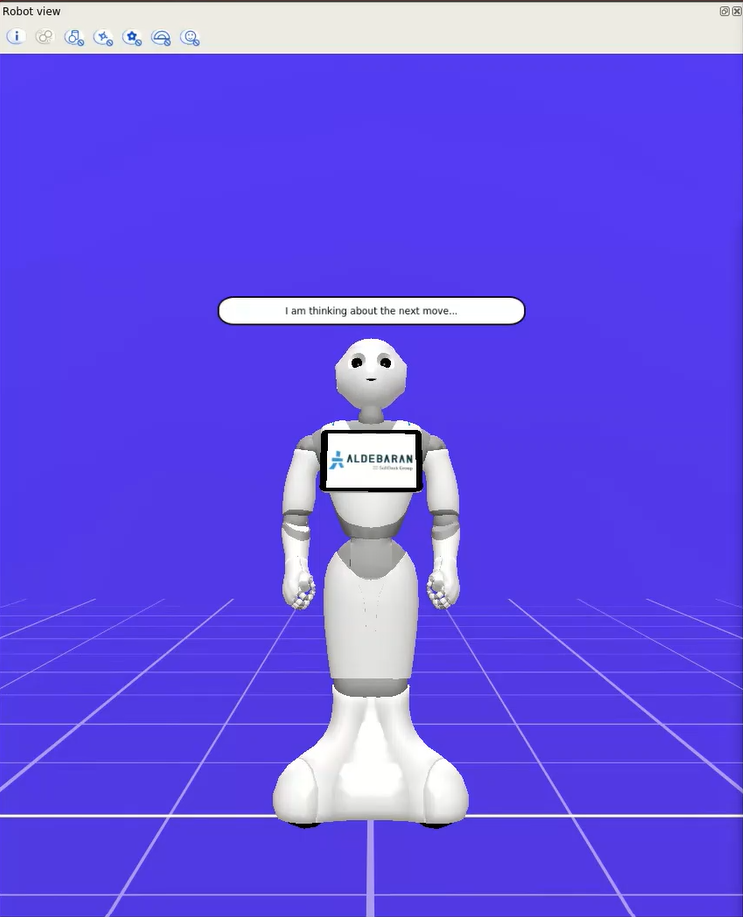
\includegraphics[width=0.9\linewidth]{images/12_tocca a pepper.png}
      \caption{Pepper thinking about next move.}
    \end{subfigure}%
    \begin{subfigure}{.33\textwidth}
      \centering
      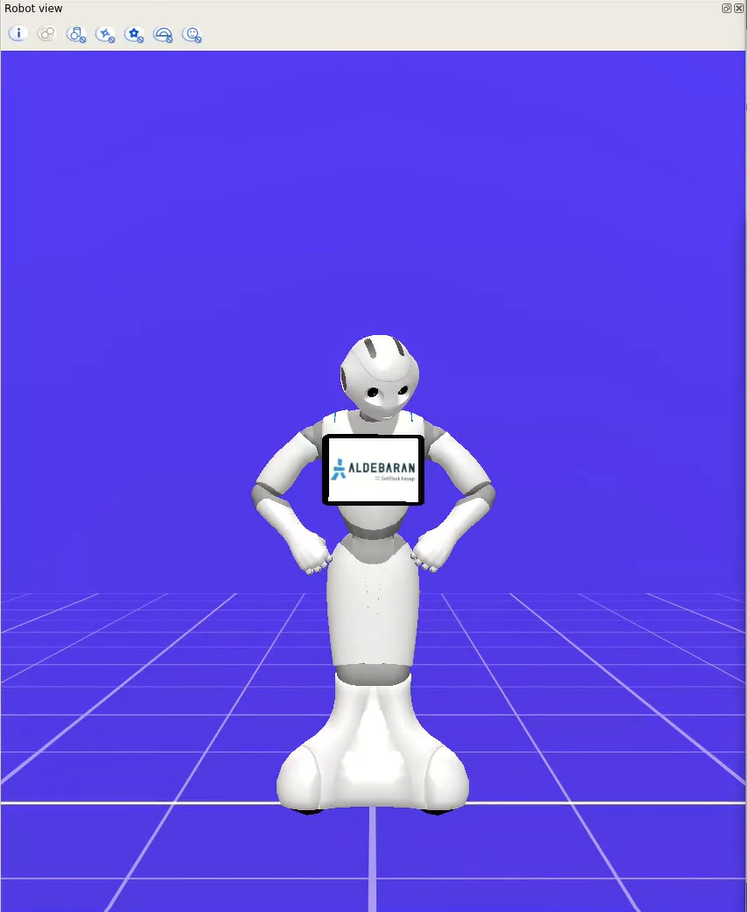
\includegraphics[width=0.9\linewidth]{images/10_pepper triste(invalida,tempo,no gioco).png}
      \caption{Pepper sad animation. }
    \end{subfigure}%
    \begin{subfigure}{.33\textwidth}
      \centering
      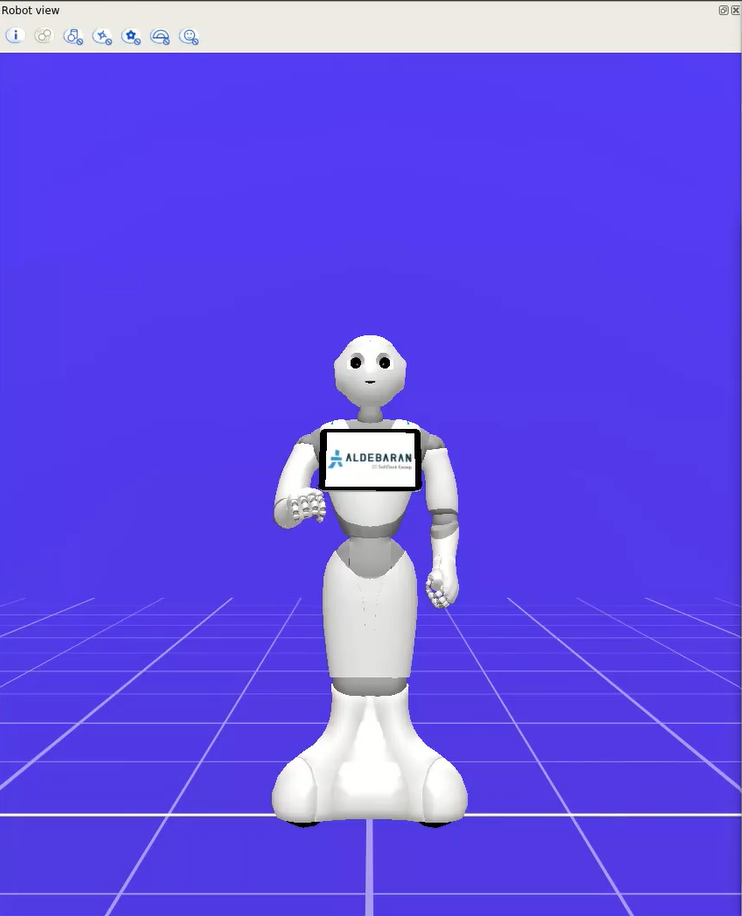
\includegraphics[width=0.9\linewidth]{images/13_mossa di pepper.png}
      \caption{Pepper move animation.}
    \end{subfigure}
    \caption{Additional Pepper reactions.}
    \label{fig:third}
\end{figure}

When the match ends thus the red car is out, Pepper first congratulates with the human and performs a victory dance. Then the robot asks if the human wants to play again the match at another level or if he wants to complete the final survey. In the first case, Pepper lets the human to choose the level suggesting to try with an higher level than the previous one (figure \ref{fig:fourth}).

\begin{figure}[H]
    \centering
    \begin{subfigure}{.33\textwidth}
      \centering
      \frame{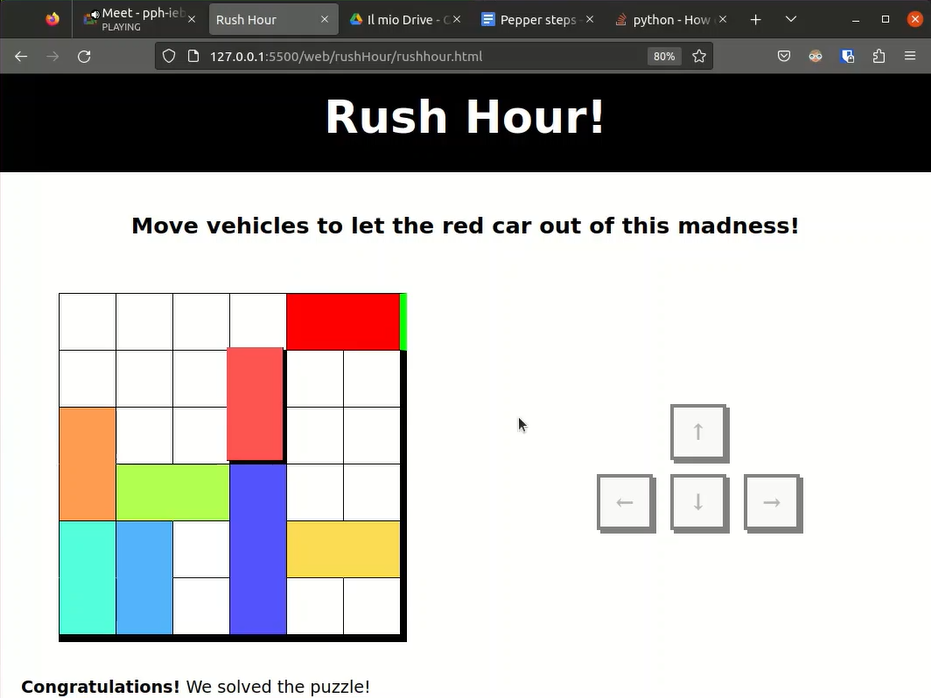
\includegraphics[width=0.9\linewidth]{images/14_vittoria.png}}
      \caption{Victory configuration.}
    \end{subfigure}%
    \begin{subfigure}{.33\textwidth}
      \centering
      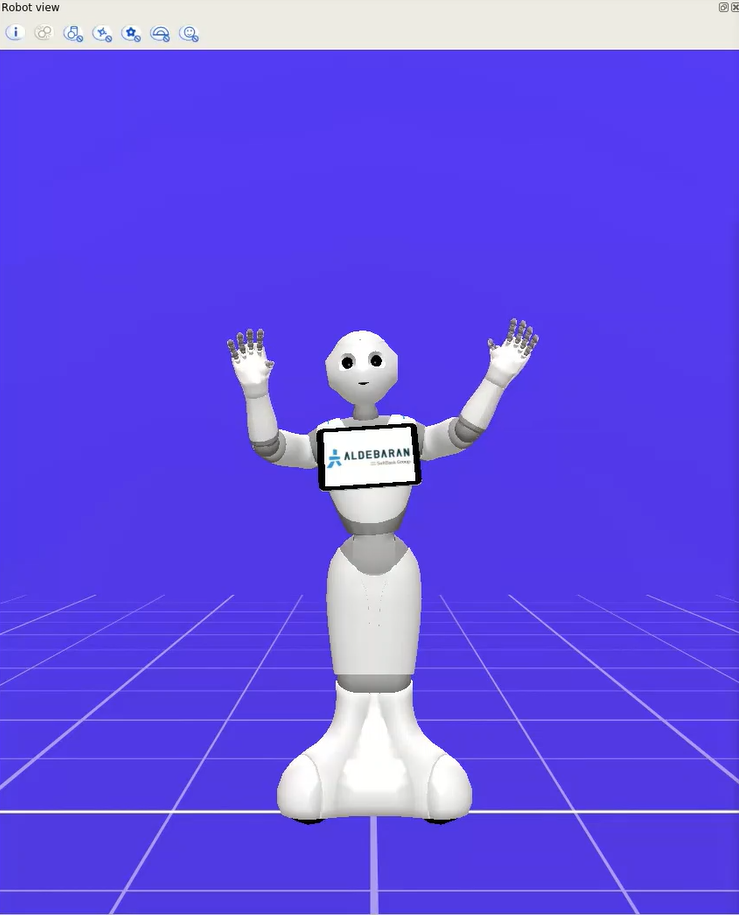
\includegraphics[width=0.9\linewidth]{images/144_vittoria.png}
      \caption{Victory dance.}
    \end{subfigure}%
    \begin{subfigure}{.33\textwidth}
      \centering
      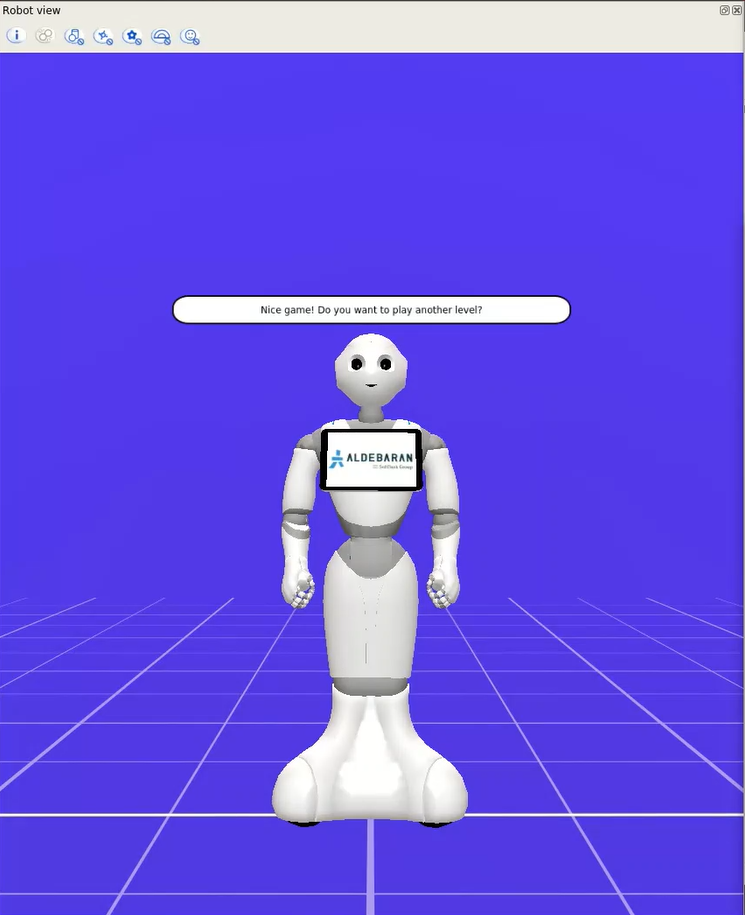
\includegraphics[width=0.9\linewidth]{images/15_vuoi giocare di nuovo.png}
      \caption{New match proposal.}
    \end{subfigure}
    \newline
    \begin{subfigure}{.33\textwidth}
      \centering
      \frame{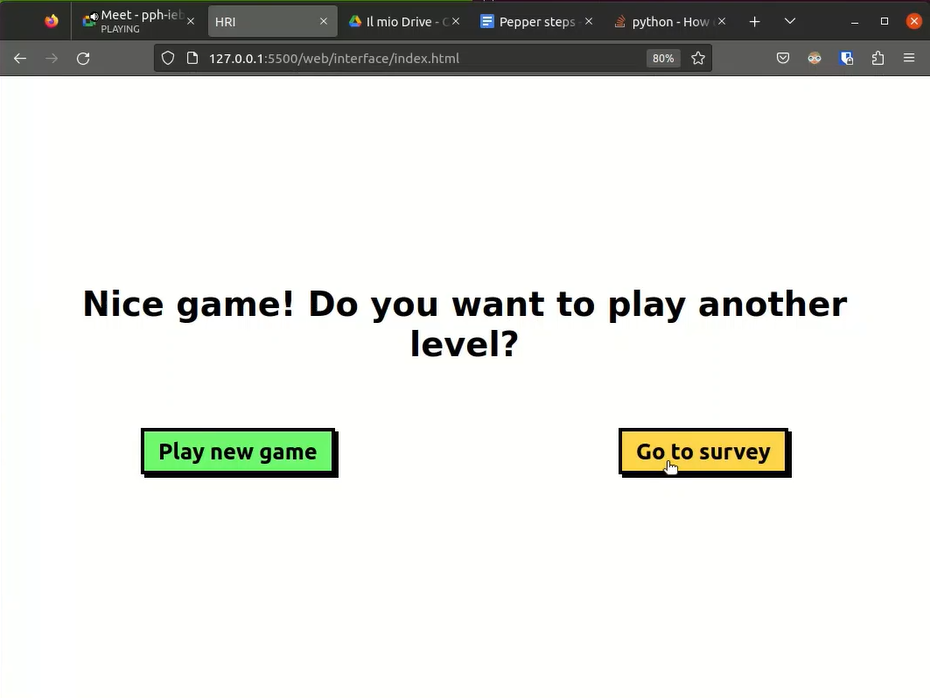
\includegraphics[width=0.9\linewidth]{images/16_vuoi giocare di nuovo.png}}
      \caption{Final choices.}
    \end{subfigure}%
    \begin{subfigure}{.33\textwidth}
      \centering
      \frame{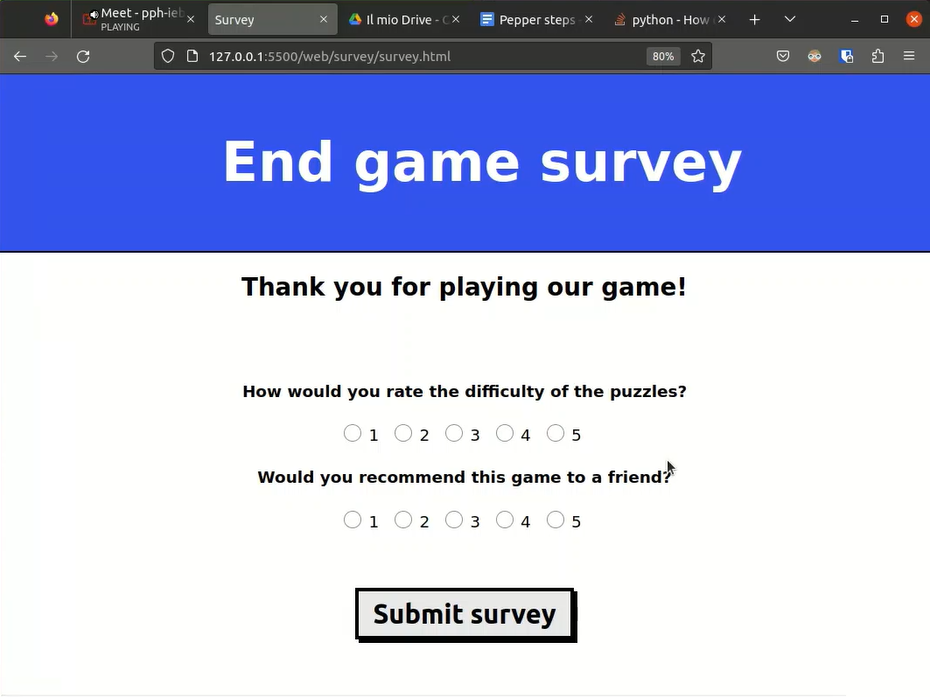
\includegraphics[width=0.9\linewidth]{images/17_sondaggio.png}}
      \caption{End game survey.}
    \end{subfigure}%
    \begin{subfigure}{.33\textwidth}
      \centering
      \frame{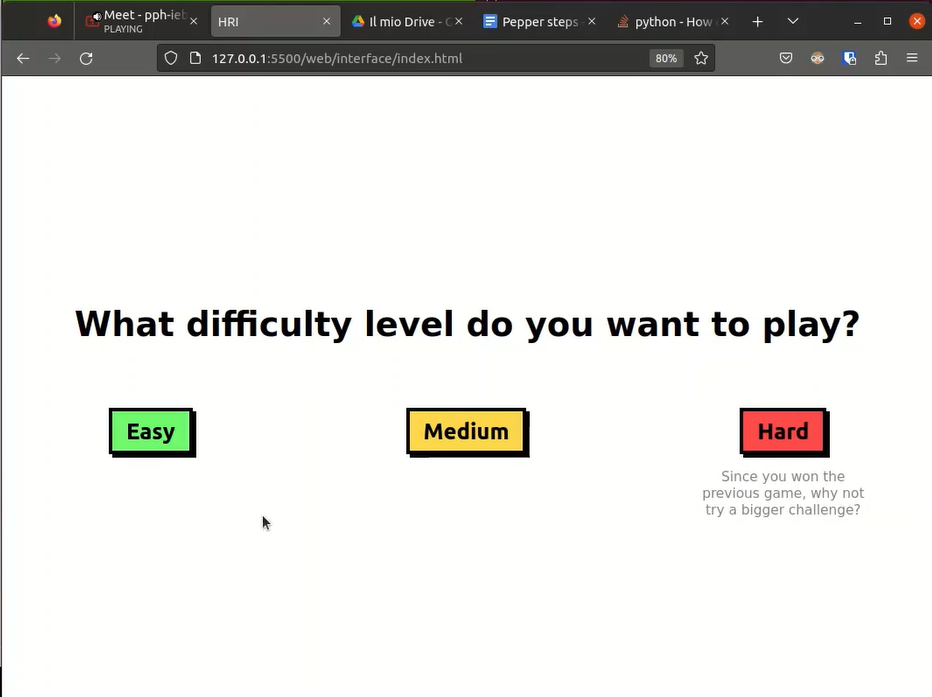
\includegraphics[width=0.9\linewidth]{images/20_seleziona livello e consiglio.png}}
      \caption{Next level selection plus suggestion.}
    \end{subfigure}
    \caption{Final interaction steps.}
    \label{fig:fourth}
\end{figure}

\noindent The results obtained using the simulated Pepper robot are shown in a demonstrative video that is publicly available at the following link: \url{https://youtu.be/QCYhiQG2Sl4}.

%* conclusions (what did you learn, how was your experience in developing the project, what can be done to further extend the functionalities and improve the effectiveness of the project) both for HRI and RA
\section{Conclusions}
\indent In recent years we are witnessing a significant increase in the use of technologies related to robotics and artificial intelligence. The fields involved in this process and in which such technologies operate are many: ranging from entertainment for elderly people, to education for children, care and many others. It's important, in fact, to ensure that these technologies help to increase the well-being of society, in order to guarantee and pave the way for progress. \\
\noindent Developing this project has been very interesting from many points of view: on the one hand it was inviting to develop a communication process that was able to make the simulated robot interact with the human via an interface, on the other hand it was interesting to understand how to implement in the best possible way the robot's behavior with that of the human and therefore understand how the robot should manage its movements, gestures and dialogues in order to ensure the best possible experience for the human. The significant aspect on which we focused on is on the way in which robot is perceived and seen by human: we want the robot to be a source of help and entertainment for the user and we want also that the human feels comfortable during the interaction with the robot.

\noindent We think that our work can be further extend in different ways in both HRI and RA aspects:
\begin{itemize}
    \item We could introduce some heuristics to make the planner faster in computing a solution to the problem. Some possible heuristics for the Rush Hour game are:
    \begin{itemize}
        \item The distance of the red car from the exit: it is an admissible heuristic since the number of actions we need to do in order to get to a goal state is at least the distance of the red car from the exit (it could be more as we might need to move some vehicles). So this heuristic does not overestimate the actual number of actions and thus is admissible.
        \item The number of cars blocking the way to the exit: it is an admissible heuristic since the number of blocking cars is lower or equal to the distance of the red car from the exit, and thus lower or equal to the number of actions we need to do.
        \item  The distance of the red car from the exit + the number of blocked blocking cars: it is an admissible heuristic since the actual number of steps to the goal is at least the distance of the red car from the exit (in order to drive it to the exit) + the number of blocked blocking cars as every such car adds a movement of the car that’s blocking it and a movement of the car itself.
    \end{itemize}
    \item We could test our project on a physical robot thus we could test the software part about sensing (e.g. sonars and speech) and we could use also the led of Pepper's eyes to improve the human-robot interaction.
    \item We could use the survey compiled by the human during the interaction with Pepper in order to make some studies. Moreover we could save the username in a database and if the human has already played Rush Hour alongside Pepper, the system would remember him having already a profile.
    \item We could add a facial recognition system in order to improve the interaction with the human since the robot would be able to look in the direction of the user.
\end{itemize} 

\indent In general, this project not only showcases the potential of the new technologies but also emphasizes the importance of creating robots that can engage and interact with humans in a social context. The ability of the robot to engage in a fun game like Rush Hour with a human player demonstrates the potential for robots to enhance human experiences and provide companionship, particularly for individuals who may be isolated or in need of social interaction. As we continue to advance the capabilities of robots, we can expect to see further exciting developments in the field of robotics that will continue to enhance our lives and change the way we interact with technology.



\bibliographystyle{unsrt}
\newpage
\bibliography{MyBibliography}

\end{document}



